\section{Methods}
\label{sec:methods}

In this section, we present our matrix-matrix multiplication. We then explain further modifications to the triple matrix multiplication (\ref{eq:rap}) that are part of the AMG setup process.

\subsection{Matrix-Matrix Multiplication}
\label{sec:matmult}

%\subsubsection{Computation}
%\label{sec:comp}
We design a divide and conquer approach to perform the sparse \mm\ in a node-local fashion. The key idea is to perform simple tasks while recursing, having efficient memory access, and to perform the multiplication for small chunks where the resulting matrix can fit into an appropriate cache. For clarity of presentation, we assume that the data is available locally and discuss it as a serial implementation. Shared memory parallelism is added in a straightforward manner.
%We have implemented \mm~ in a recursive fashion.
%We split the matrices recursively in two ways: split by half based on the matrix size and based on number of nonzeros. First we explain the algorithms performing splitting based on the matrix sizes.

To perform the multiplication
\begin{equation}
    Ax = b
\end{equation}
we keep splitting the matrices horizontally or vertically based on row and column size of $A$. The recursive function, \recmm, includes three cases:
\begin{enumerate}
 \item Case 1: Stop the recursion: perform the multiplication.
 \item Case 2: $A$ is horizontal. Split $A$ and $B$.
 \item Case 3: $A$ is vertical. Split $A$ and $B$.
\end{enumerate}

\subsubsection{Case 1}
\label{sec:case1}
By splitting sparse matrices recursively, we will have more and more zero rows and columns in the resulting sub-matrices. So, using row size and column size of those sub-matrices is not very helpful. Instead, we use nonzero rows and nonzero columns.
At the start of the recursive function, the number of nonzero rows of A ($A\_nnz\_row$) and nonzero columns of B ($B\_nnz\_col$) are being computed. A threshold for $\nnzsz = A\_nnz\_row \times B\_nnz\_col$ is set. Our algorithm has a profiling step where it empirically determines the appropriate threshold by running several test cases. On the machines we used,  $20M$ was chosen as the threshold. We continue splitting the matrices until the threshold is reached. Then, we preform the multiplication. We have implemented two methods for this case: dense data structure and hashmap.

%First method uses a dense matrix.
%The matrices are ordered as column-major.
% In the first method, a dense matrix of size $\nnzsz$ is initialized to $0$. \mr{explain better:}Each nonzero of $B$ is multiplied by its corresponding nonzero of $A$ and the result will be added to the corresponding index in the dense matrix. At the end, we go through the dense matrix and add the nonzeros to the final multiplication matrix.
When performing the multiplication, at least one of the matrices, typically the output, needs random access as it is accumulating the results. Given that the divide and conquer approach has reduced the size of the output matrix, the first approach is to keep a temporary buffer for dense matrix storage. Each nonzero of $B$ is multiplied by its corresponding nonzero of $A$ and the result will be added to the corresponding index in the dense matrix. As long as the dense matrix is small enough to fit within the L2 cache, we should get good performance. At the end of the multiplication, we traverse the dense matrix and extract the non-zeros as a sparse matrix. This approach works well as long as the resulting matrix is dense. 

When $\nnzsz$ gets larger, it becomes inefficient to traverse the whole dense matrix and check for nonzeros in the final stage. To solve this issue, we use an efficient hashmap to achieve similar results without the $\mathcal{O}(n^2)$ overhead of extracting the non-zeros from the dense matrix. The entry's index is the key and its value is the hashmap's value. When we want to add the multiplication of nonzeros of $A$ and $B$ to the hashmap, we check if the index exists in the map. If it exists the value is being added to the existing one's. Otherwise a new entry will be added to the hashmap. Clearly, there is an overhead to this approach that needs to be balanced against the overheads associated with the dense representation. 

\begin{figure}[tbh]
 \centering
 %\Description{Description}
 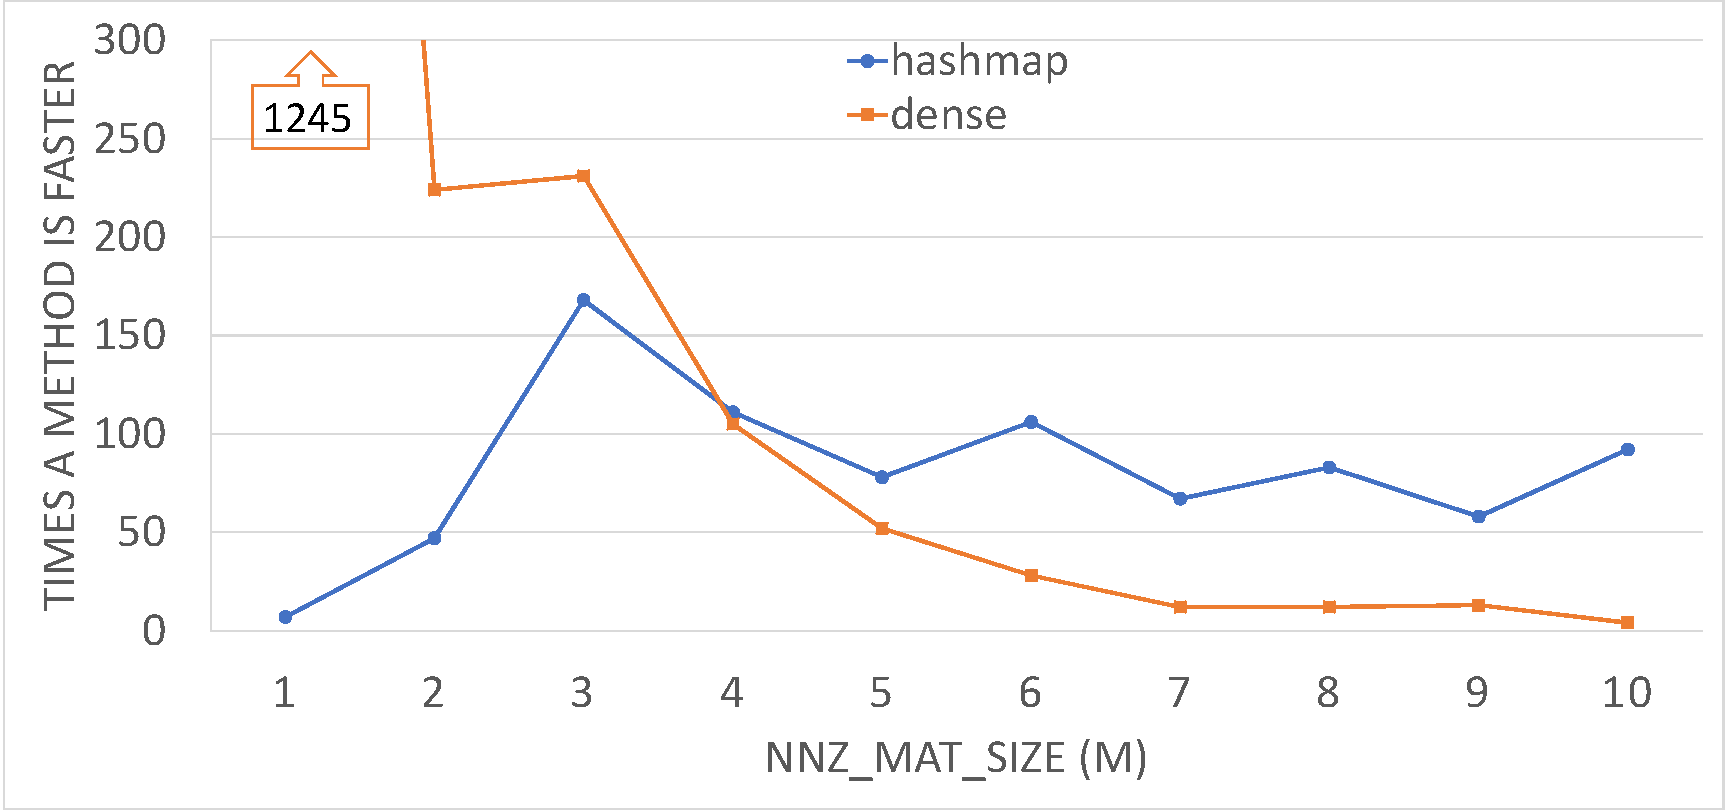
\includegraphics[width=8.5cm,height=4cm]{./figures/lap60_range.pdf}
 \caption{Comparison between dense structure method with hashmap to compute coarse matrix $Ac = R \times A \times P$, in which $A$ is the 3D Poisson problem of size $216k$. The plot shows the number of times each method is faster than the other one in intervals of $1M$ for $\nnzsz$.}
 \label{fig:lap60}
 \Description{}
\end{figure}

In Figure~\ref{fig:lap60}, we compare the two methods for computing coarse matrix $Ac = R \times A \times P$, in which $A$ is the 3D Poisson problem of size $216k$. For $0 \leq \nnzsz \leq 10M$, in $1M$ steps, we compare the two methods in order to develop an efficient hybrid algorithm. For instance, the first point indicates that the dense structure is better than hashmap in $1245$ cases for all multiplications such that $0 \le\ \nnzsz < 1M$. For the lower range the dense representation is better and for the higher range the hashmap is significantly faster. Figure~\ref{fig:eco} shows the same experiment for matrix ID $1882$ from SuiteSparse (Florida) Matrix Collection, which is a sparse matrix of size $1M$ and $5M$ nonzero.

A combination of these two methods would give us the best performance across different matrix structures and densities. The dense method is being used for the lower range and the hashmap for the higher range.
We have done a series of experiments to determine the threshold when to switch between the two methods. Figures~\ref{fig:lap60} and \ref{fig:eco} suggest to use the dense structure method when $0 \le\ \nnzsz < 4M$ and use hashmap for the rest. We noticed that when hashmaps are better, the difference time between the two methods on average is higher. In other words, on average, $n$ times performing hashmap is faster than $n$ times using the dense structure. So empirically, we found $1M$ to be a good estimate for switching between the two methods.

\begin{figure}[tbh]
 \centering
%\Description{Description}
 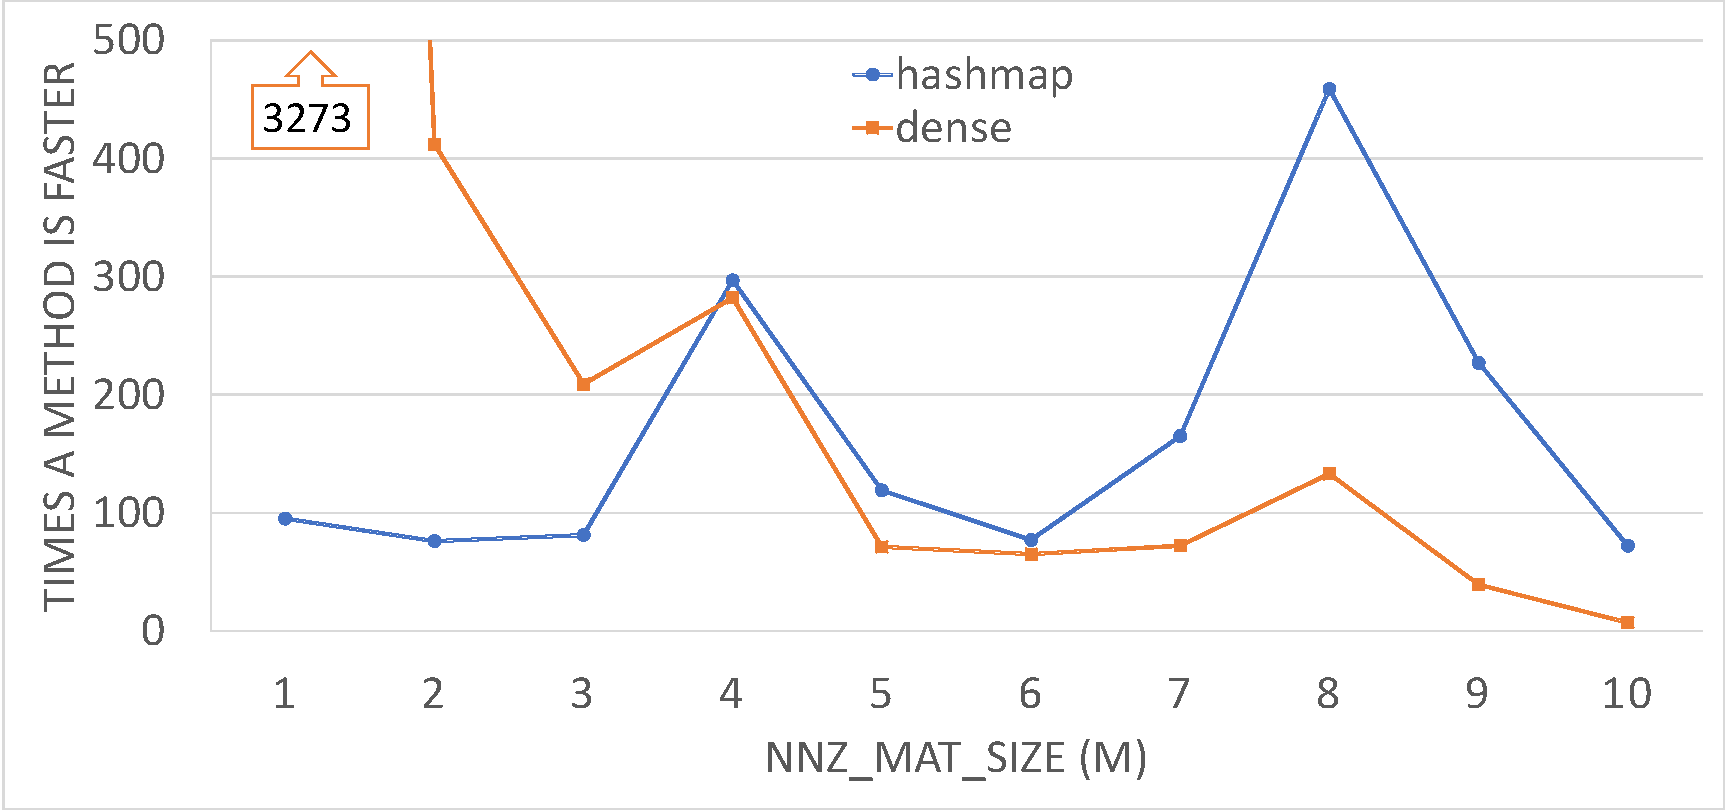
\includegraphics[width=8.5cm,height=4cm]{./figures/eco_range.pdf}
 \caption{Comparison between dense structure method with hashmap to compute coarse matrix $Ac = R \times A \times P$, in which $A$ is matrix ID $1882$ from SuiteSparse (Florida) Matrix Collection. The plot shows the number of times each method is faster than the other one in intervals of $1M$ for $\nnzsz$.}
 \label{fig:eco}
 \Description{}
\end{figure}

\begin{figure}[tbh]
 \centering
 %\Description{Description}
 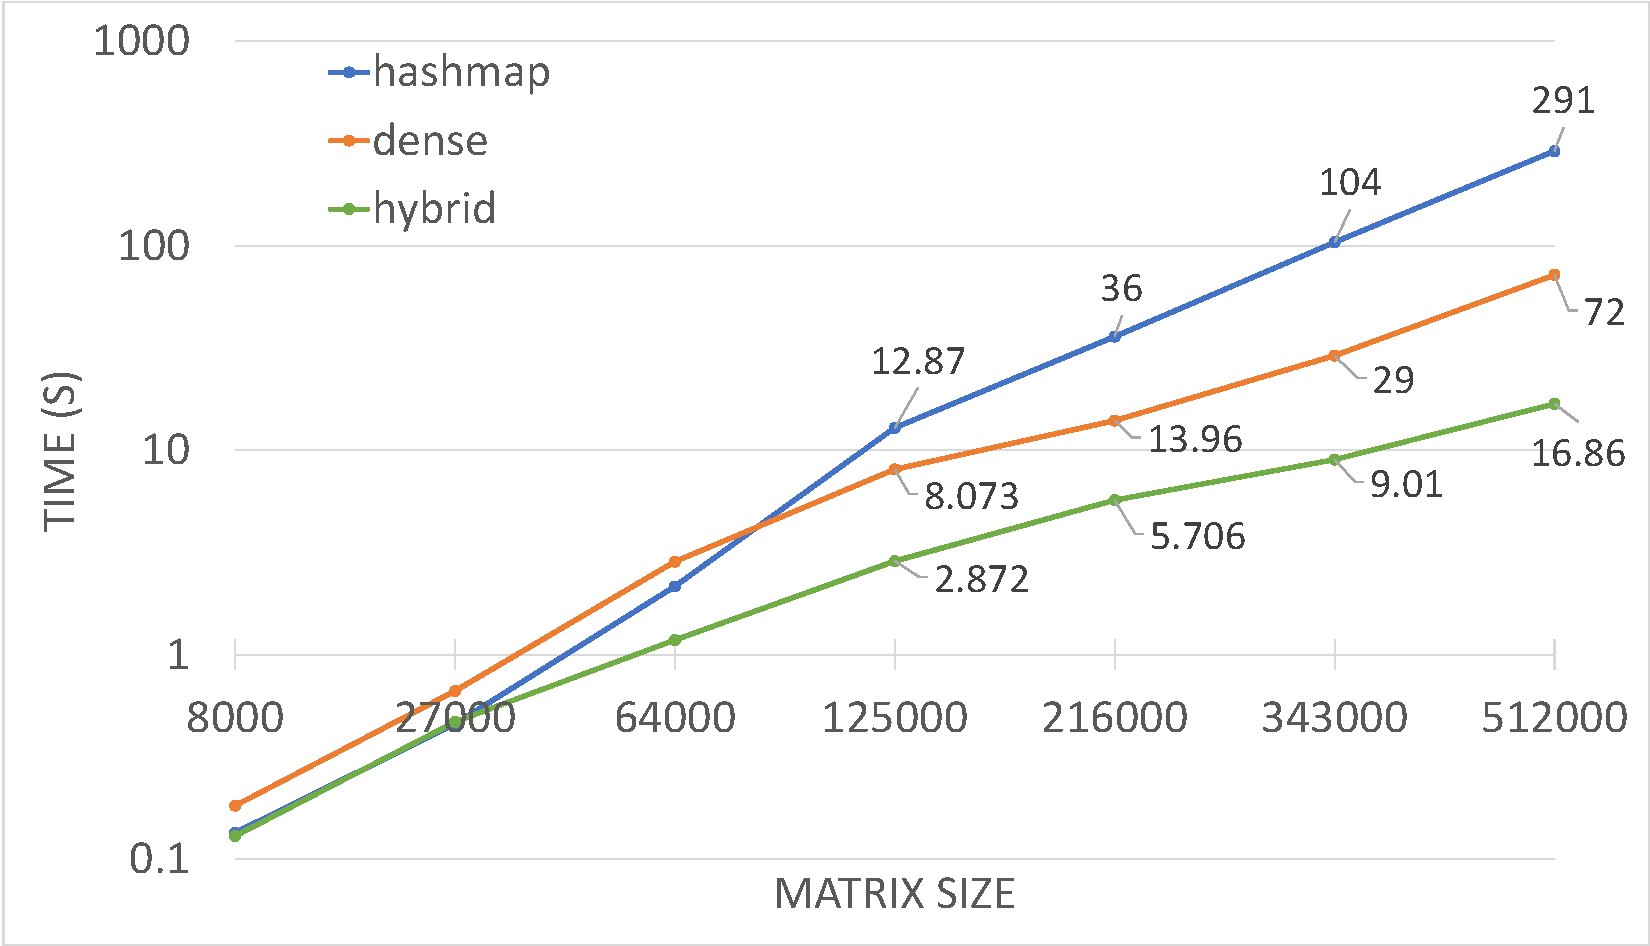
\includegraphics[width=8.5cm,height=5cm]{./figures/mix.pdf}
 \caption{Comparison between the three methods to do Case 1: only using hashmap, only using the dense structure, and the hybrid method. They are used as Case 1 to compute the first coarse matrix (the triple multiplication) on 7 matrices (3D Poisson) of different sizes.}
 \label{fig:mix}
 \Description{}
\end{figure}

Figure~\ref{fig:mix} compares the hybrid method with the basic two methods. We have compared the three approaches on different sizes of 3D Poisson problem, ranging from $8k$ to almost half a million. For instance, for the case where the matrix is of size $512k$, computing the first coarse matrix (performing the triple matrix) takes $291s$ if only hashmap is used for Case 1, takes $72s$ if only the dense structure is used and finally takes almost $17s$ when the hybrid approach is utilized for Case 1.


\subsubsection{Case 2}
\label{sec:case2}
When A is horizontal, i.e. its row size is less than or equal to its column size, we halve A by column based on its column size (Figure~\ref{fig:case2_left}). Since row size of B equals column size of A, we halve B by row, so it will be a split similar to A, but horizontally.
Then, the \recmm~ will be called twice, once on $A1$ and $B1$, and again on $A2$ and $B2$ (Algorithm~\ref{alg:case2}). The results of the two multiplications will need to be added together at the end. It means, there will be entries for the result matrix with the same index, e.g. multiple entries with $(10, 20)$ as the index. We call these entries \textit{duplicates}. Since there will be numerous nested recursive calls, we avoid doing adding duplicate at this stage. After the first recursive function is finished, we will perform a sorting and then add the duplicates only once at the end.

\begin{figure}[tbh]
    \centering
    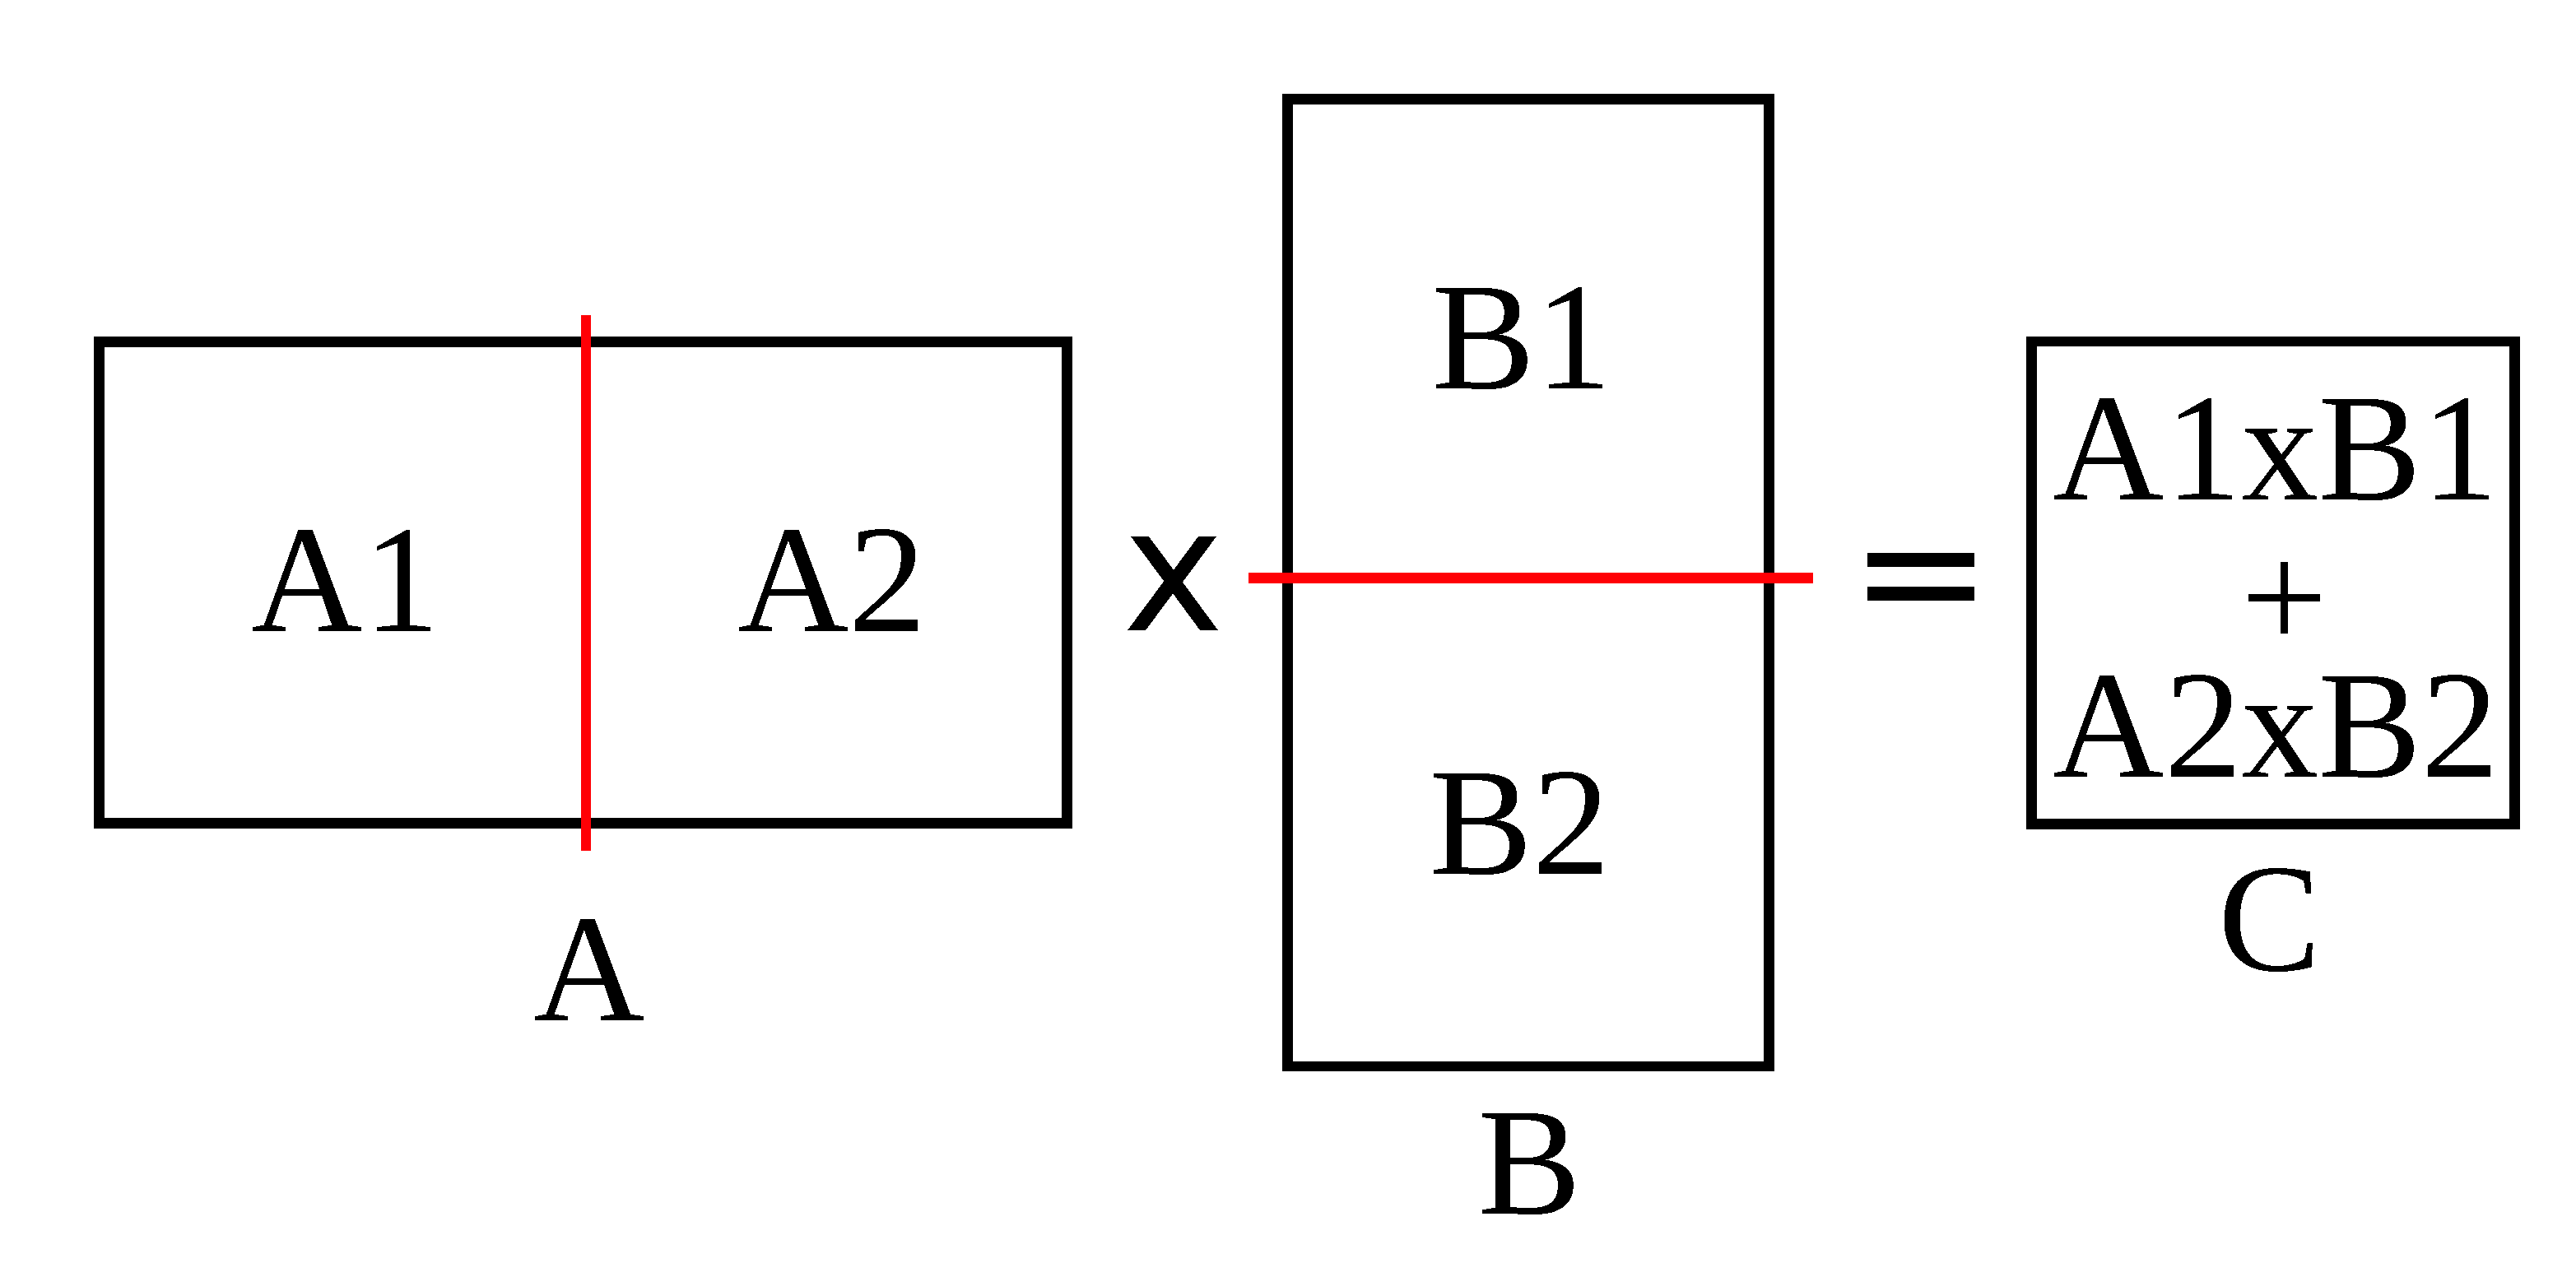
\includegraphics[width=4.5cm,height=2.3cm]{./figures/case2_001.pdf}
    \caption{Case 2: When A is horizontal, split A by column and B by row. Call the recursive function twice.}
    \label{fig:case2_left}
    \Description{}
\end{figure}

\begin{figure}[tbh]
    \centering
    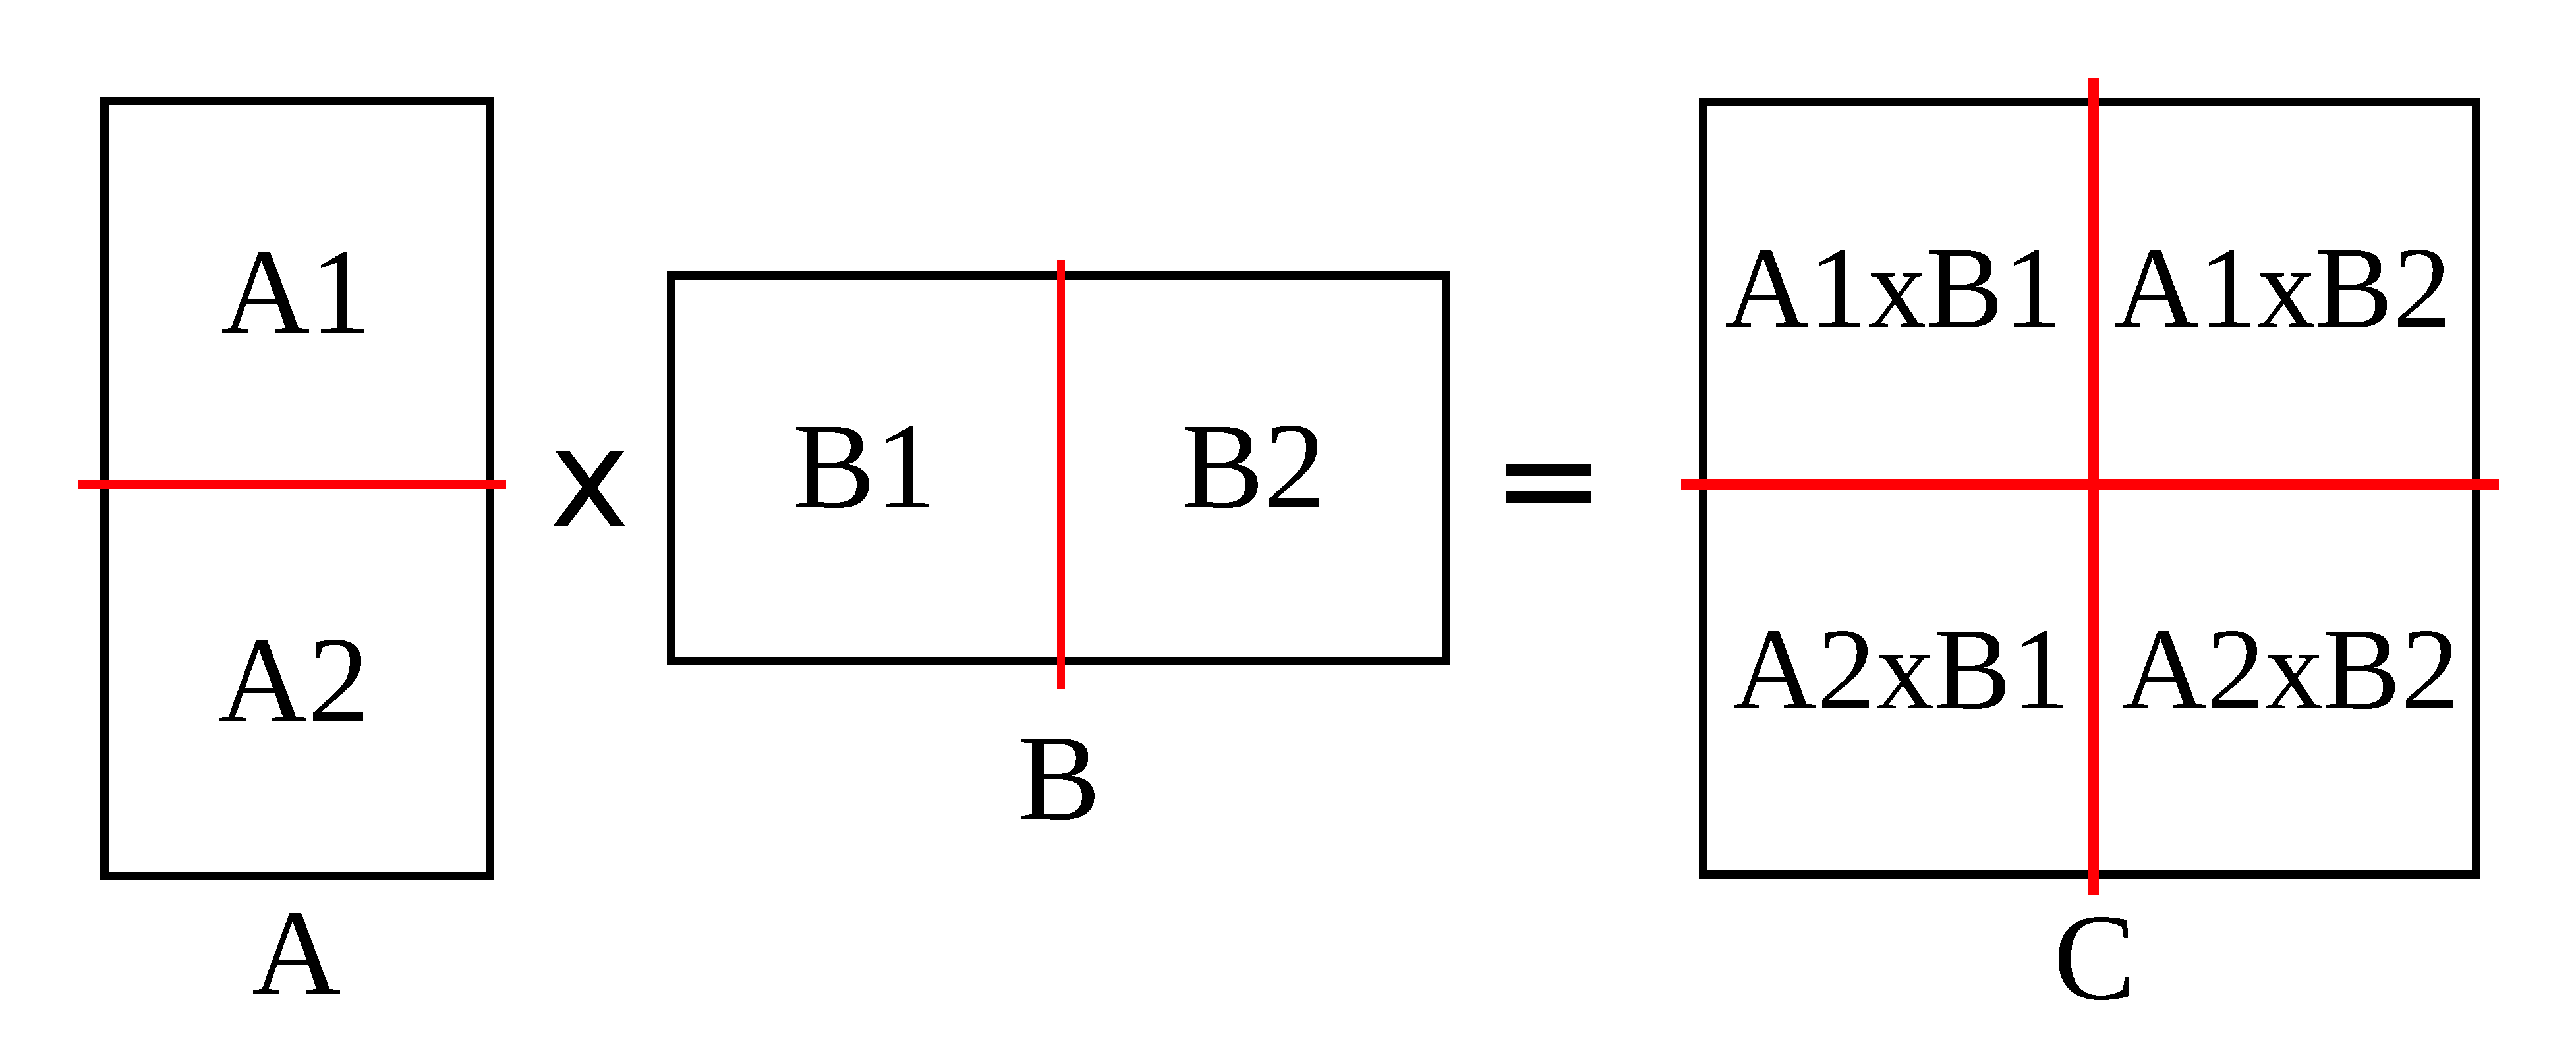
\includegraphics[width=5.5cm,height=2.3cm]{./figures/case3_001.pdf}
    \caption{Case 3: When A is vertical, split A by row and B by column. Call the recursive function four times.}
    \label{fig:case3}
    \Description{}
\end{figure}

\begin{algorithm}[tbh] 
  %\footnotesize
  \caption{Case 2: $C = \recmm2(A, B)$} \label{alg:case2} 
  \begin{algorithmic}[1]
    \Require $A$, $B$
    \Ensure  $C$
    \State $(A1, A2) = \spc(A)$
    \State $(B1, B2) = \spr(B)$
    \State $C \leftarrow \recmm(A1,B1)$
    \State $C \leftarrow \recmm(A2,B2)$
    %\State $C \leftarrow \textsc{mergesort}(C1, C2)$
  \end{algorithmic}
  \Description{}
\end{algorithm}

\subsubsection{Case 3}
\label{sec:case3}
When A is vertical, i.e. its row size is greater than its column size, we halve A by row based on its row size and halve B by column (Figure~\ref{fig:case3}). In contrary to the previous case, the column size of B is not related to row size of A, so they are split independently. This time the \recmm~ will be called four times (Algorithm~\ref{alg:case2}).  Although we have 4 recursive calls in this case, but there is no duplicates at the end, which makes this case more efficient than Case 2 for the total time, because it is faster to do the sorting and adding duplicates at the end on a smaller set of entries. 

\iffalse
\begin{figure}[tbh]
 \centering
 %\Description{Description}
 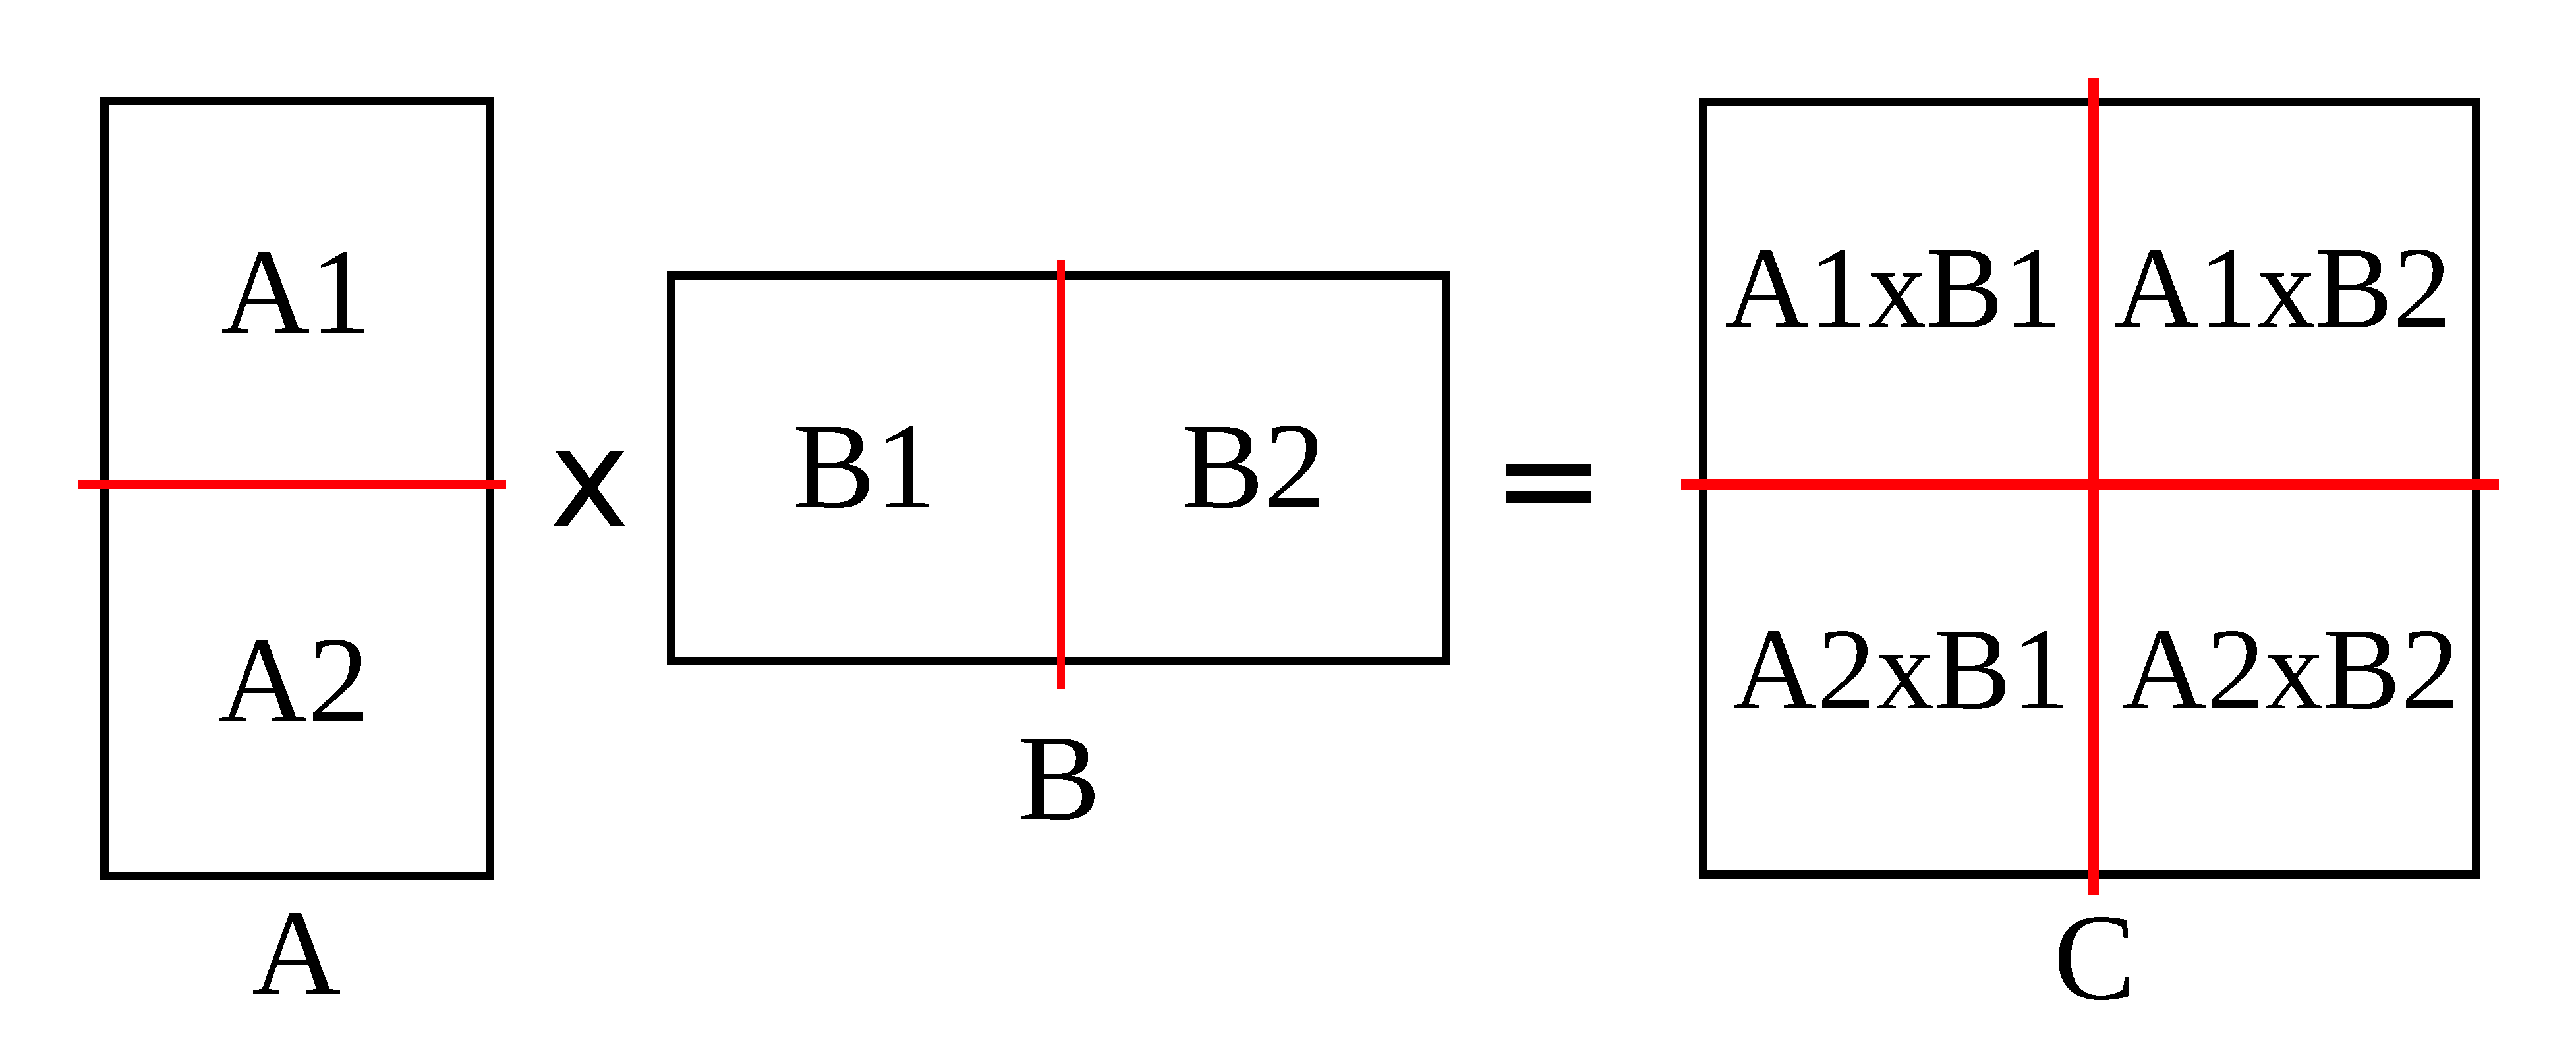
\includegraphics[width=6cm,height=2.5cm]{./figures/case3_001.pdf}
 \caption{Case 3: When A is vertical, split A by row and B by column. Call the recursive function four times.}
 \label{fig:case3}
\end{figure}
\fi

\begin{algorithm}[H] 
  %\footnotesize
  \caption{Case 3: $C = \recmm3(A, B)$} \label{alg:case3} 
  \begin{algorithmic}[1]
    \Require $A$, $B$
    \Ensure  $C$
    \State $(A1, A2) = \spr(A)$
    \State $(B1, B2) = \spc(B)$
    \State $C \leftarrow \recmm(A1,B1)$
    \State $C \leftarrow \recmm(A2,B1)$
    \State $C \leftarrow \recmm(A1,B2)$
    \State $C \leftarrow \recmm(A2,B2)$
    %\State $\textsc{sort}(C)$
  \end{algorithmic}
\end{algorithm}

We have also implemented splitting based on the number of nonzeros. In \textit{Case 2}, we split $A$ in a way to have half of nonzeros in $A1$, and the other half in $A2$. The same split is used for $B$. In \textit{Case 3}, we do the same, but separately for both $A$ and $B$.

\subsubsection{All together}

When all three cases work together, we have Case 2 and Case 3, that aim to divide the matrices into skinny matrices such that the resulting matrix is small. Then by using a hybrid multiplication algorithm, we get these results. These results are then accumulated and merged together. From a memory access perspective, the accumulation and merging required for Case 2 and 3 is structured access to the matrix, with the only random access happening during Case 1. This makes the overall algorithm very efficient. 

\subsection{AMG Matrix-Multiplication: Communication}
\label{sec:amg}

% To solve a large linear system 
% \begin{equation}
%  Ax = b
% \end{equation}
% using an Algebraic Multigrid approach, we scale down the system, solve it directly, then scale back the solution. To scale down the system, three different categories of matrices are being created: coarse matrices ($As$), restriction matrices ($Rs$) and prolongation matrices ($Ps$). To study how $Ps$ and $Rs$ are computed you can refer to \cite{bell2012exposing, treister2015non}. Here we focus how to compute $As$, assuming $Ps$ and $Rs$ are available. We explain how to compute the first coarse matrix, the next ones can be computed similarly.

% original text starts here 
As noted earlier, to compute the coarse matrix $Ac$, a triple matrix multiplication is performed:
\begin{equation}
 Ac = R \times A \times P
\end{equation}
with $R = P^T$ in the Galerkin approach, which we use in our implementation.
%
In this section, we explain how the communication is setup to compute the coarse matrix $Ac$, exploiting properties of the matrix structure specific to AMG. 
%
Matrices are partitioned across multiple processors by row blocks (Figure~\ref{fig:partition}). Matrices $A$ and $P$ have the same number of rows and consequently are partitioned the same way. $R$ has fewer number of rows and has a different partition. This is because coarsening need not be uniform across processes. Consequently the partitioning of the rows of $R$ could be different from that of $A$ and $P$. The triple matrix product is performed in two parts: first $A \times P$ is computed, followed by $R \times B$, where $B = A \times P$ is the result of the first multiplication. In other words, this is equivalent to performing matrix-matrix multiplications (\mm) twice.

\begin{figure}[tbh]
 \centering
 %\Description{Description}
 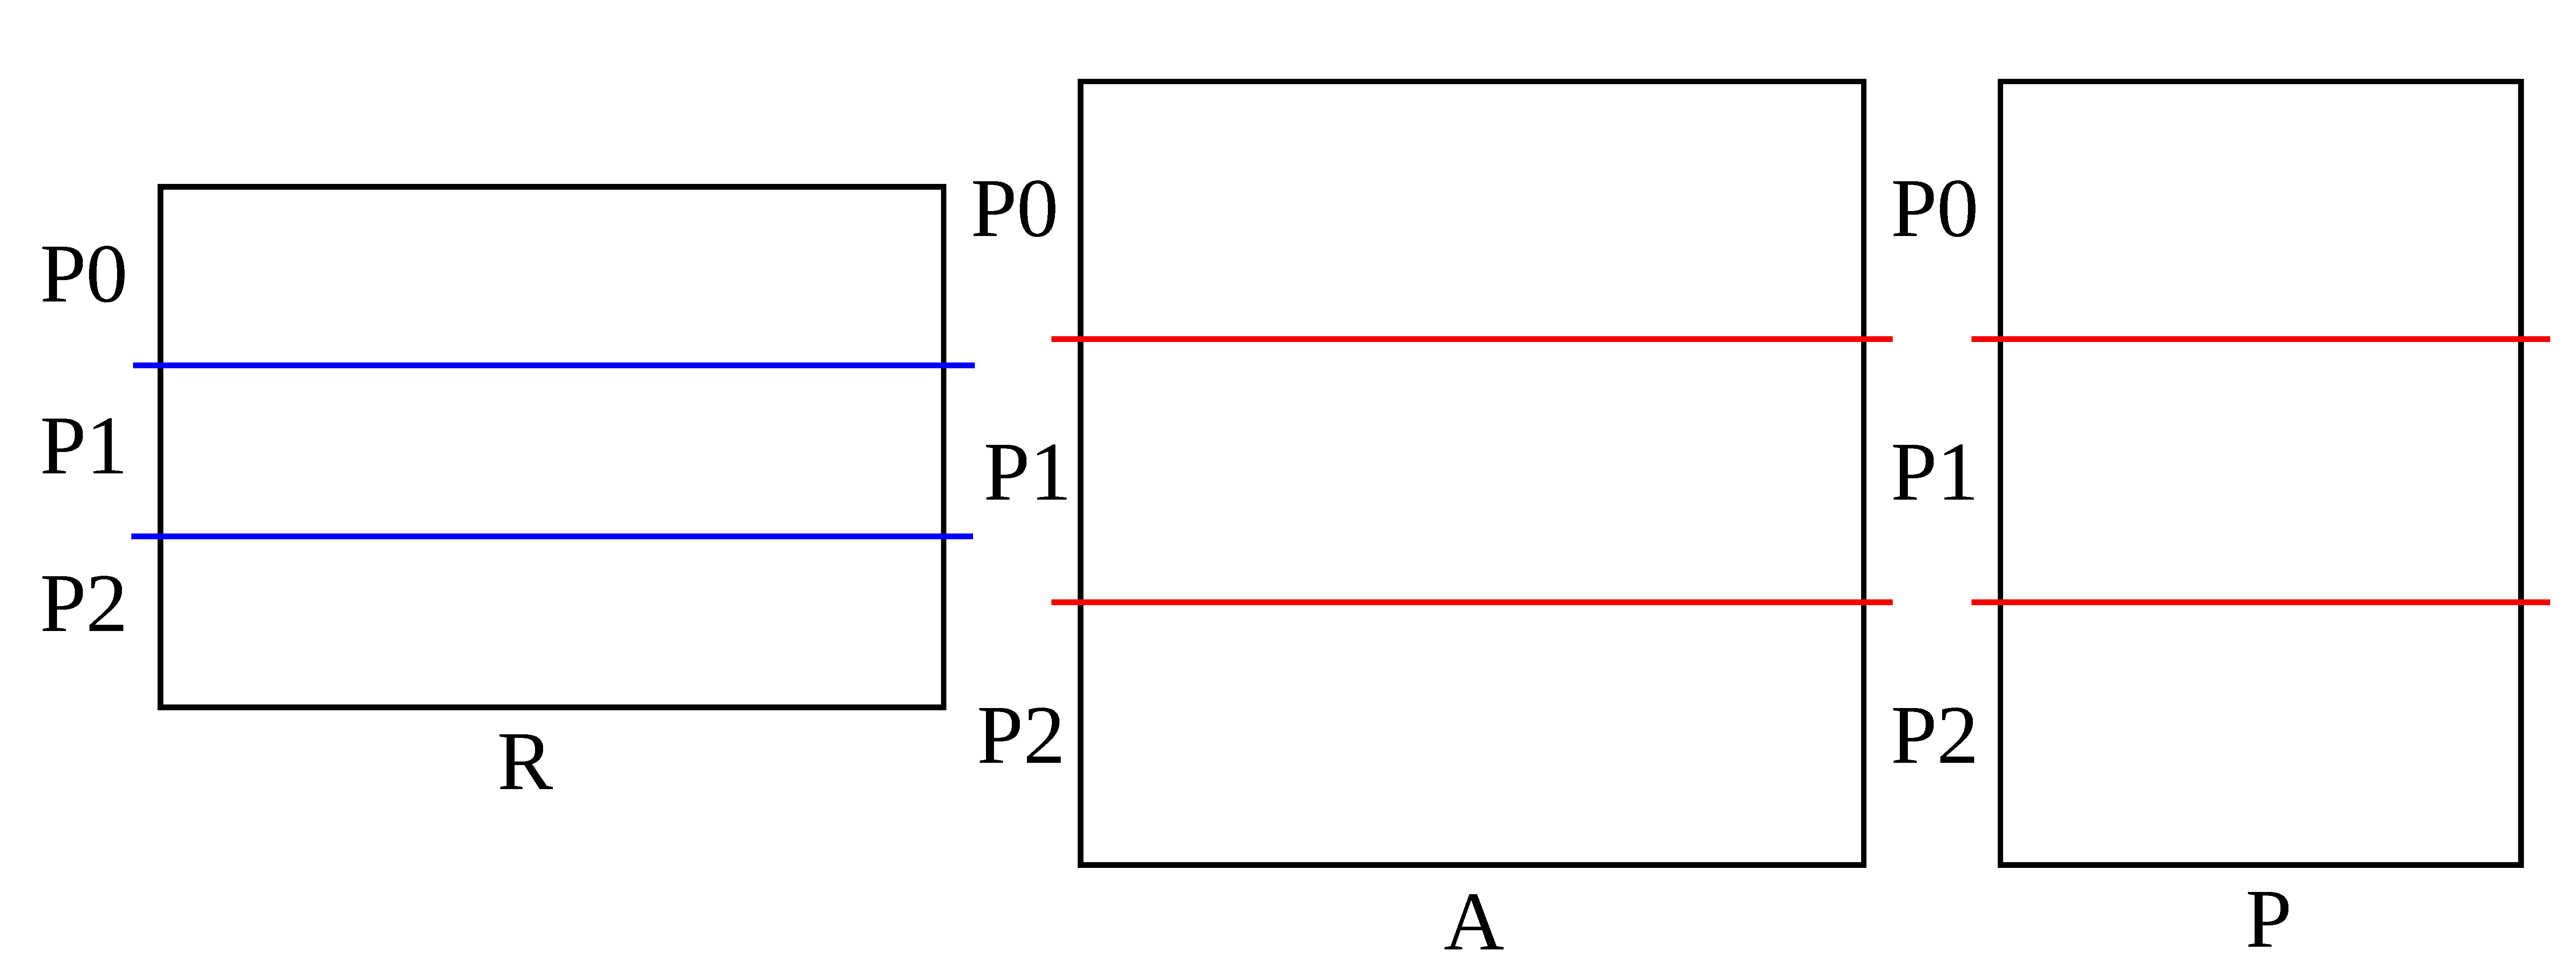
\includegraphics[width=7cm,height=2.7cm]{./figures/partition.pdf}
 \caption{Partitioning of the matrices across the processors in row blocks. $A$ and $P$ have the same partition but $R$'s is different.}
 \label{fig:partition}
 \Description{}
\end{figure}

\subsubsection{Part 1}

In this part, we explain how to compute $B := A \times P$. We assume the same partition of rows of $A$ on also its columns (red lines) since $A$ is square. For columns of $P$ we use the partition of rows of $R$ (blue lines in Figure~\ref{fig:part1b}).
Without loss of generality, let us focus on how to perform \mm ~on processor $P1$. To compute entry $B(i, j)$, we need to multiply row $i$ of $A$ with column $j$ of $P$ and add them together (since we are working with sparse matrices, we only consider the nonzeros here).

\begin{figure}[tbh]
    \centering
    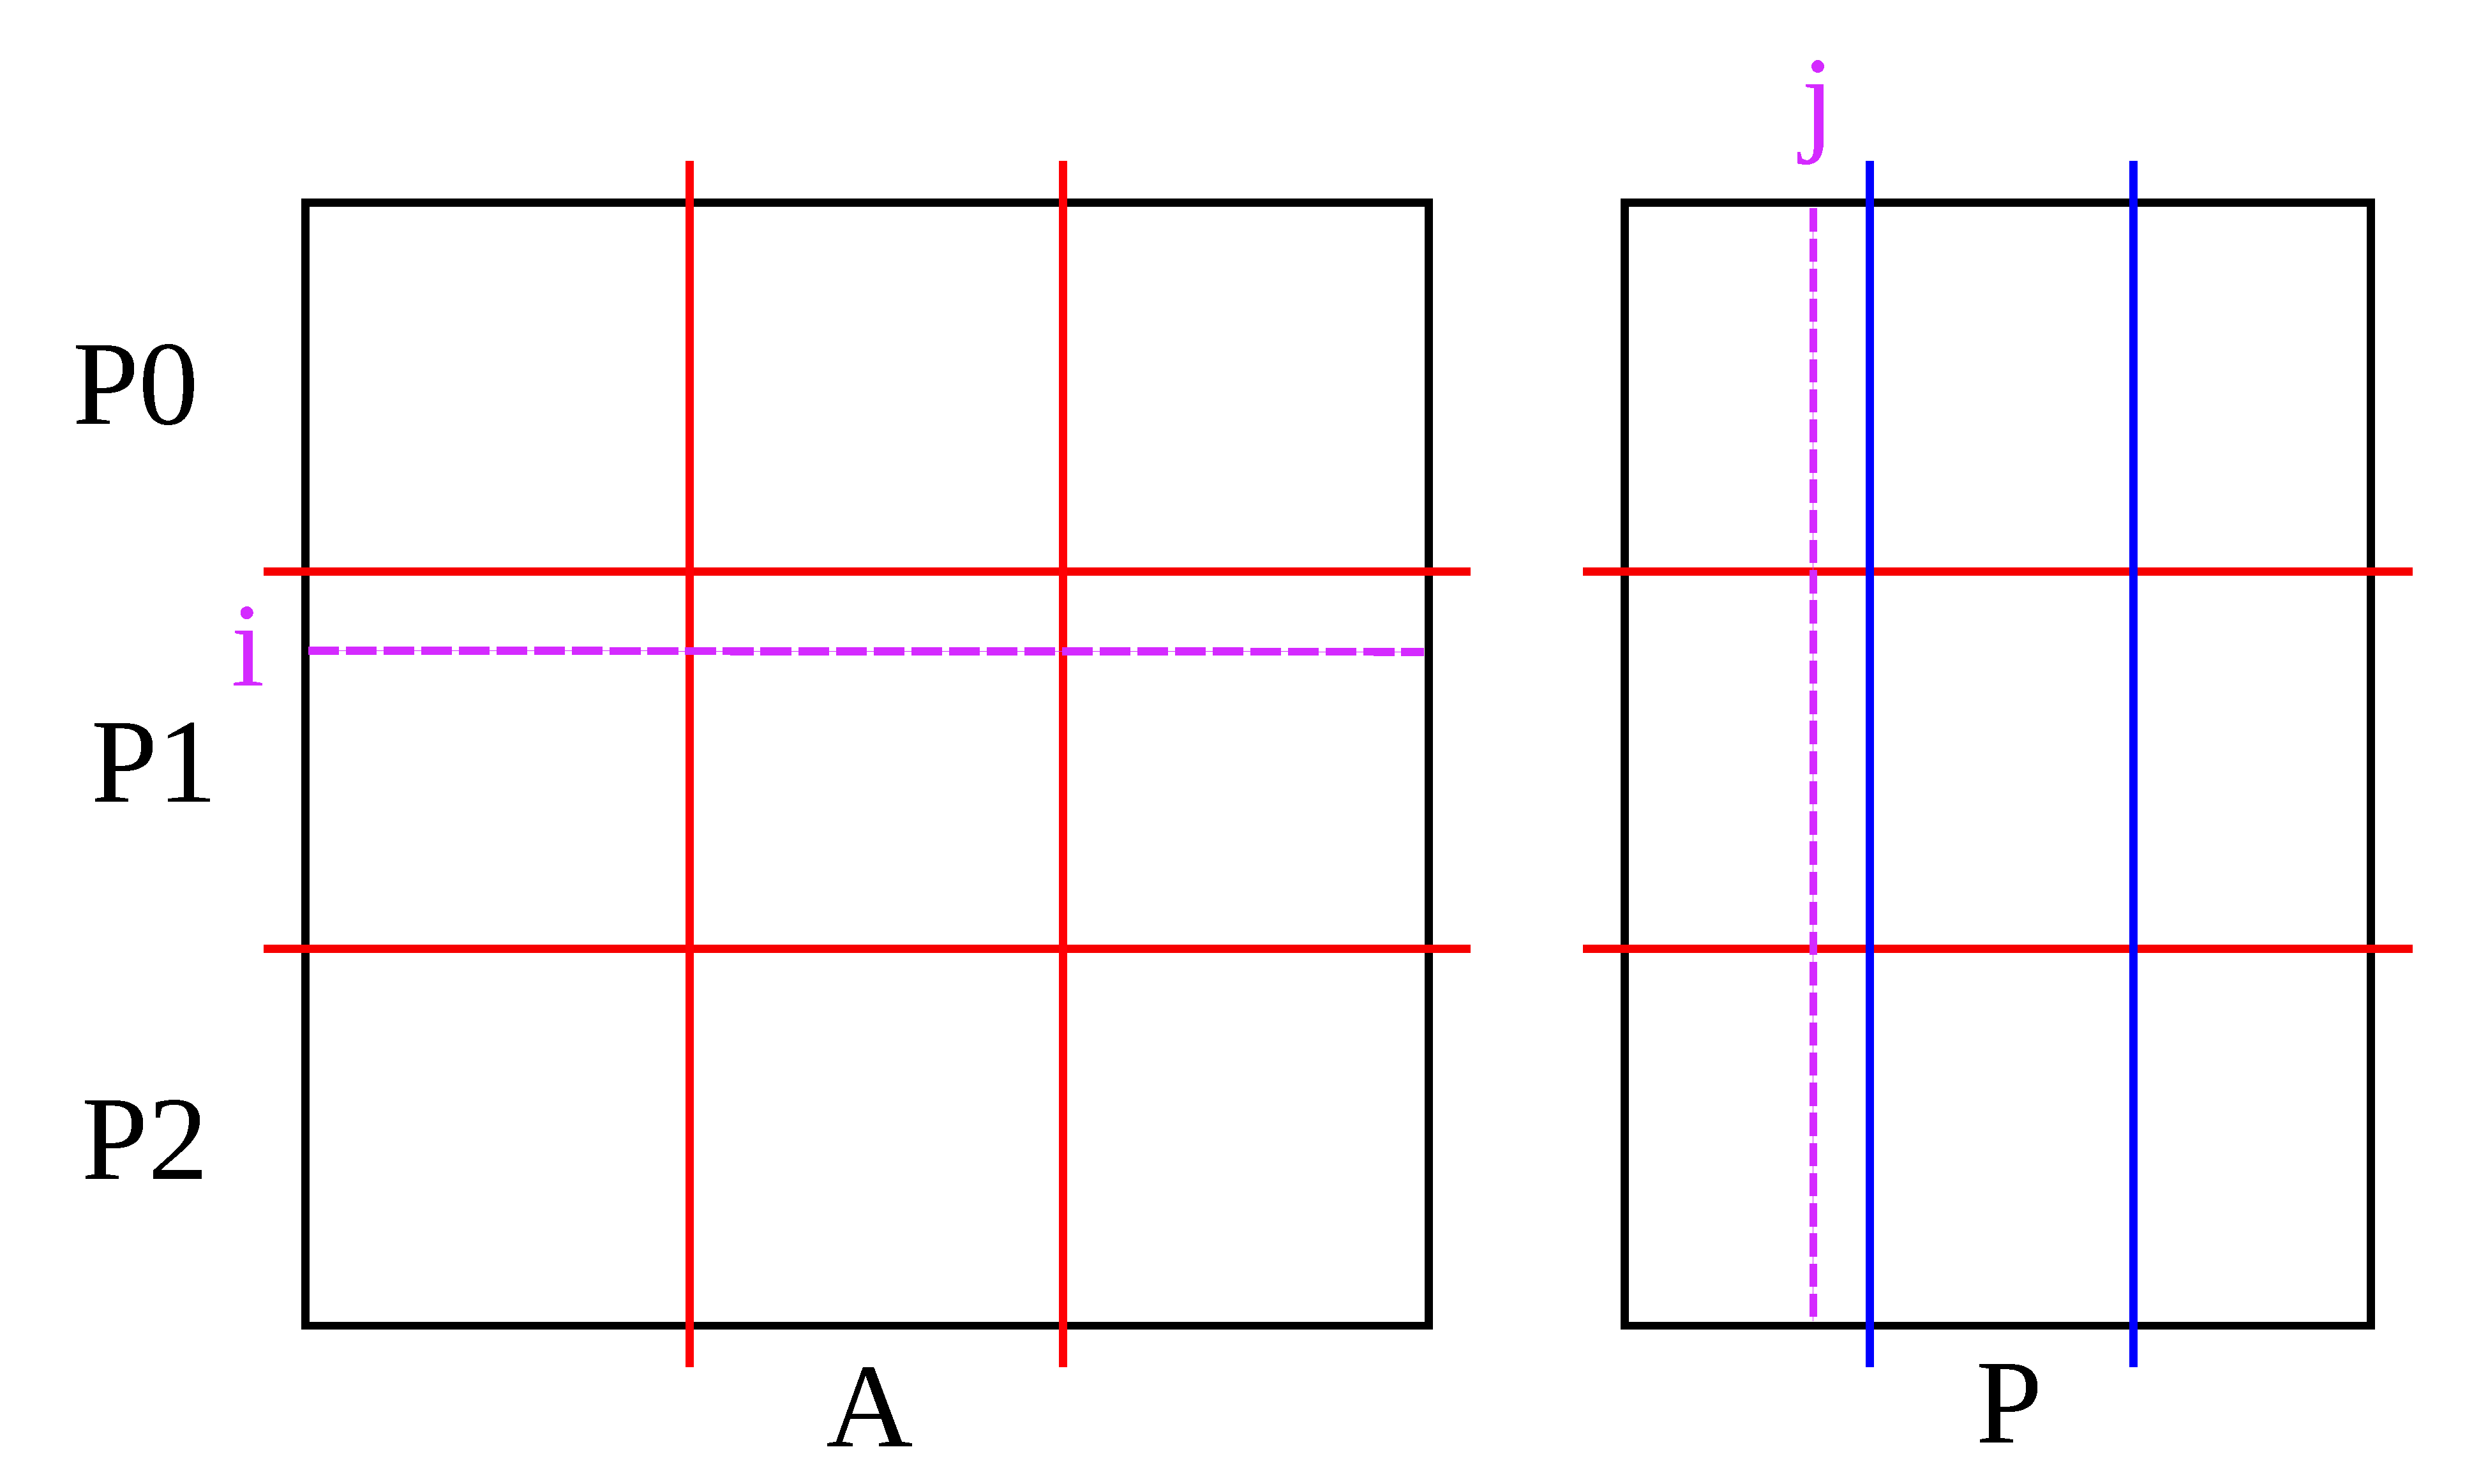
\includegraphics[width=5cm,height=3cm]{./figures/part1b.pdf}
    \caption{This figure shows how the matrices are split into sub-blocks in Part 1. Column $j$ of $P$ is stored on different processors.}
    \label{fig:part1b}
    \Description{}
\end{figure}

\begin{figure}[tbh]
    \centering
    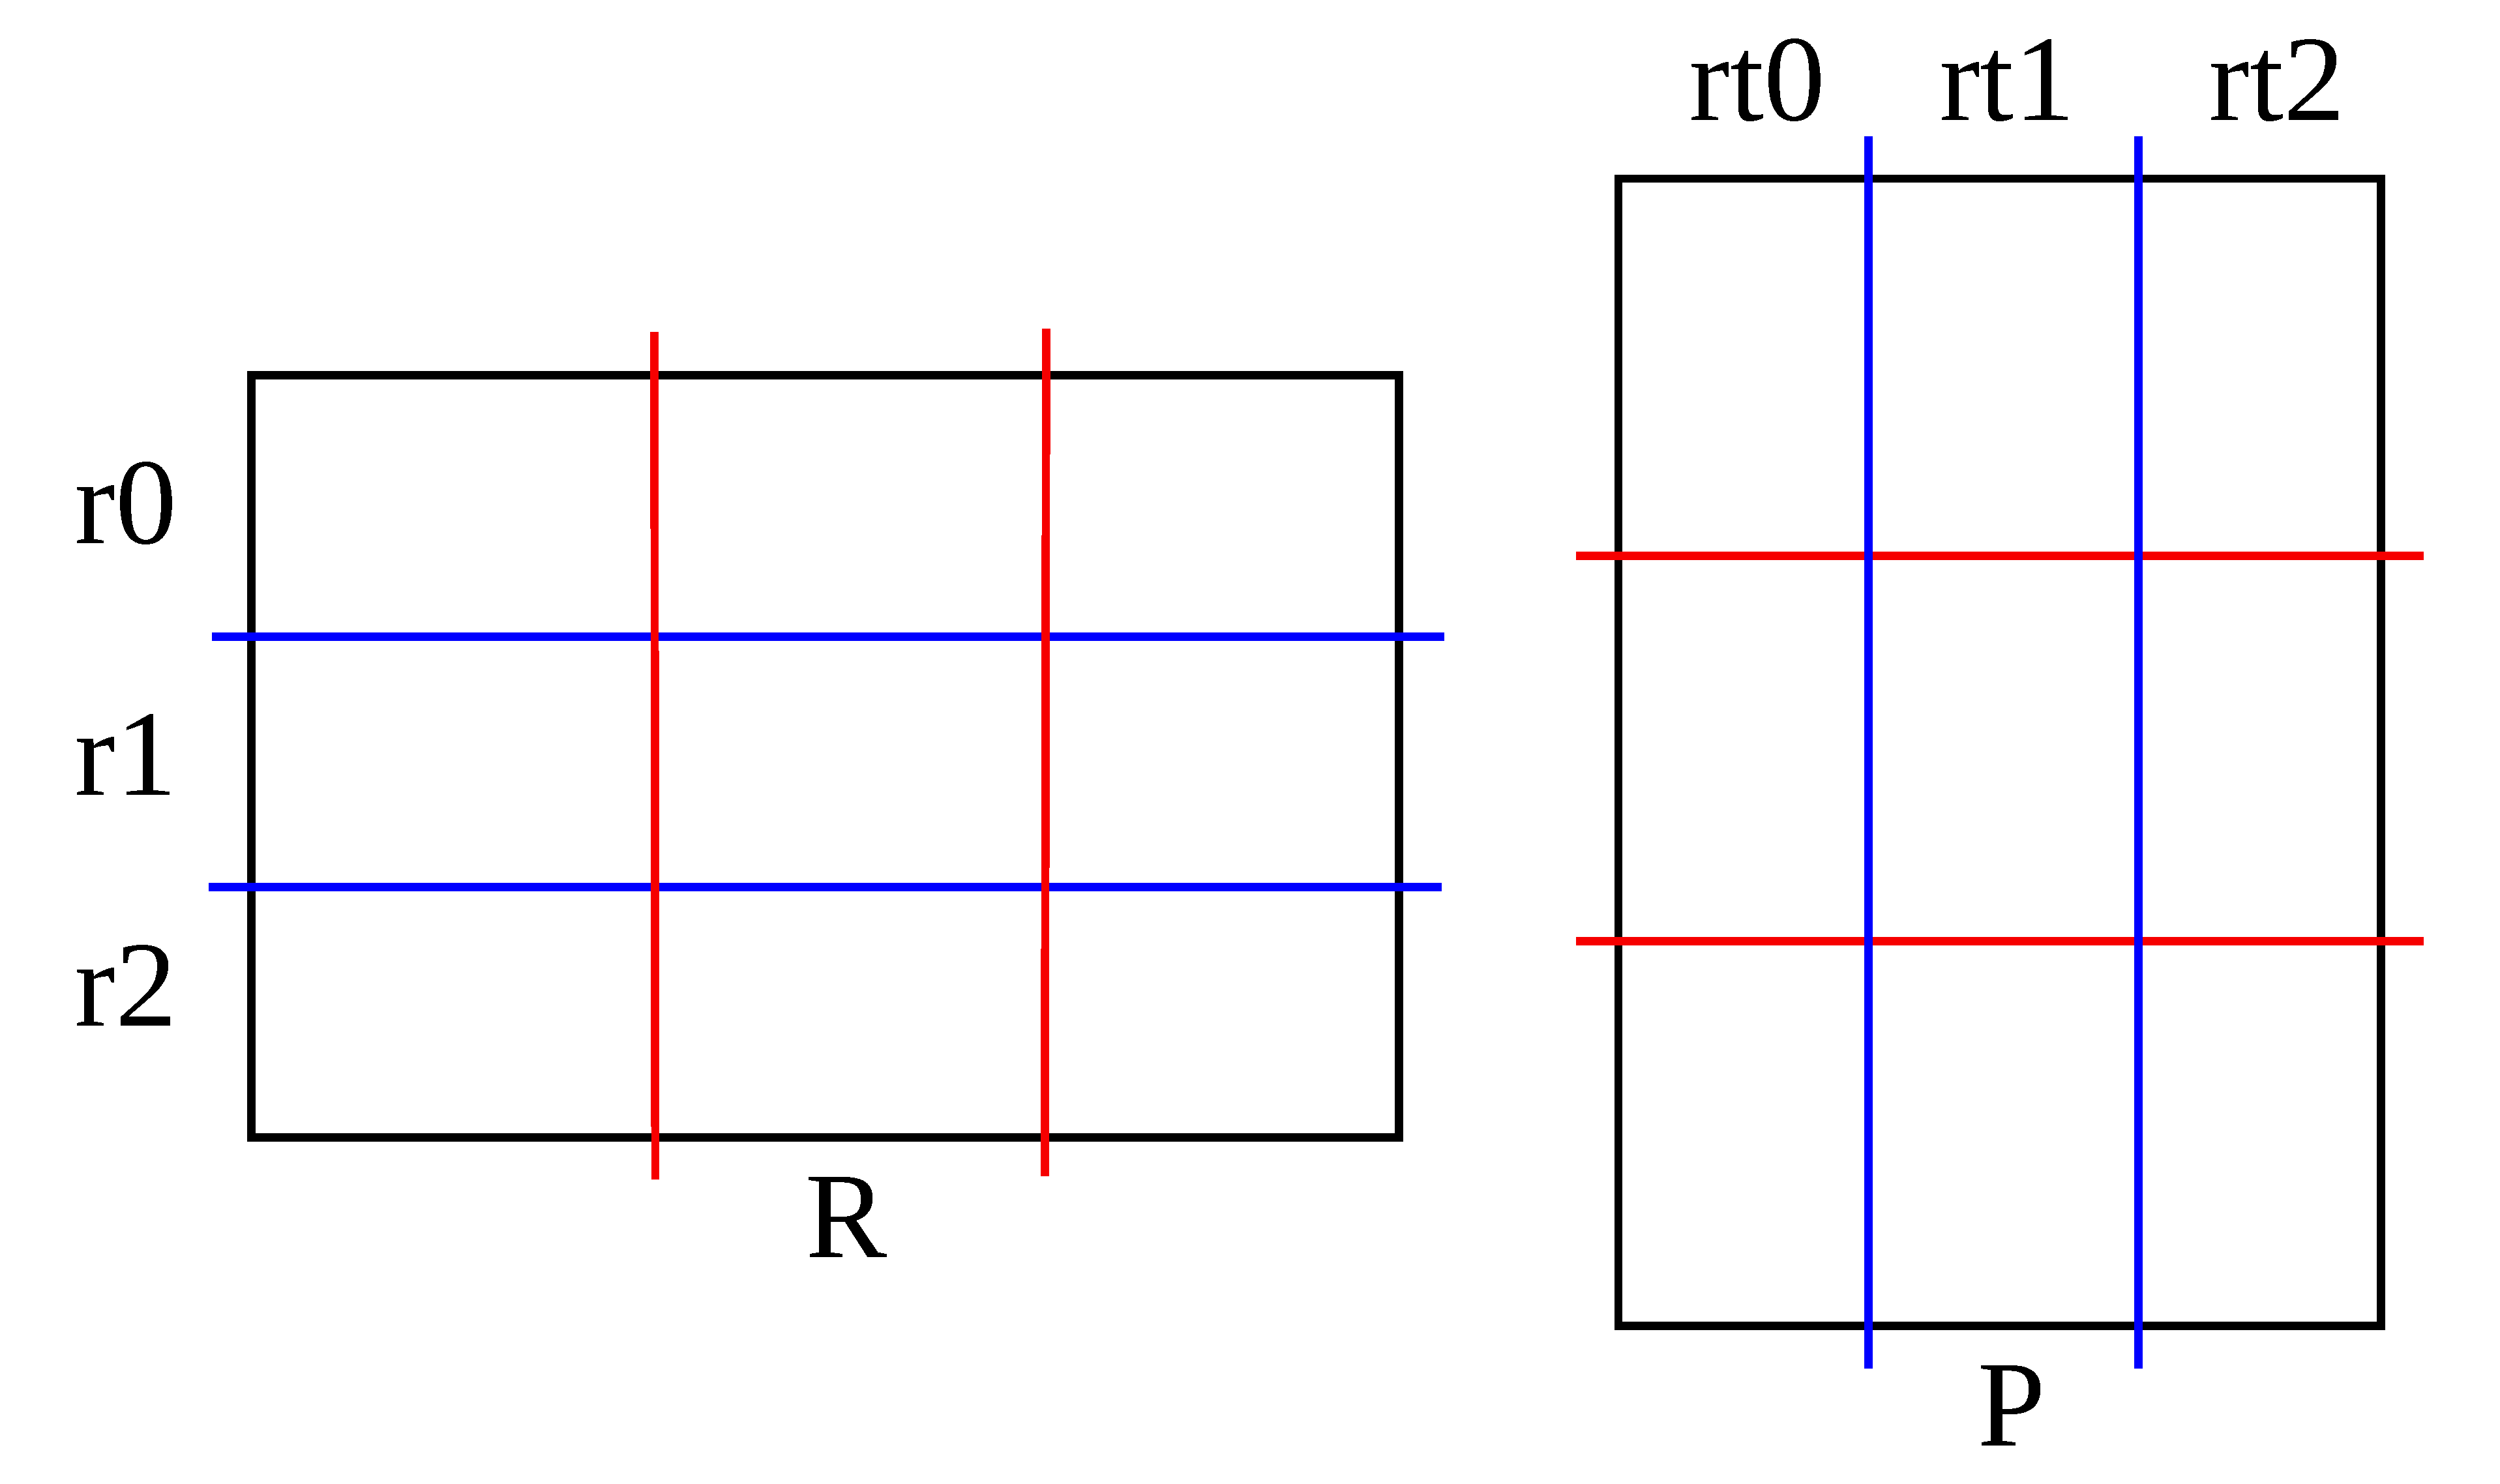
\includegraphics[width=5cm,height=2.9cm]{./figures/part1c.pdf}
    \caption{This figure shows how row blocks of $R$ are transpose of column blocks of $P$.}
    \label{fig:part1c}
    \Description{}
\end{figure}

Column $j$ of $P$ is distributed between all the processors. Therefore we need to communicate all nonzeros of that column and then perform $B_{ij} = \sum_{k} A_{ik} P_{kj}$. Since that can lead to significant communication, we make use of the fact that $R$ is the transpose of $P$ and is already available locally because of the multigrid hierarchy. We note that column blocks of $P$ (e.g. $r0$ in Figure~\ref{fig:part1c}) are actually row blocks of $R$ transposed ($rt0$, which is transpose of $r0$).

We have implemented this part in an overlapped fashion; first we do the send and receive commands (to communicate $rt$ blocks) and while this communication is being done, we perform \mm, so saving time for the communication (Algorithm \ref{alg:part1}). $B_{i}$ in the algorithm is the row block of matrix $B$ on processor $i$ and $B_{ik}$ is the sub-block result of multiplying $A_i$ with $rt_k$.

\iffalse
\begin{figure}[tbh]
 \centering
 %\Description{Description}
 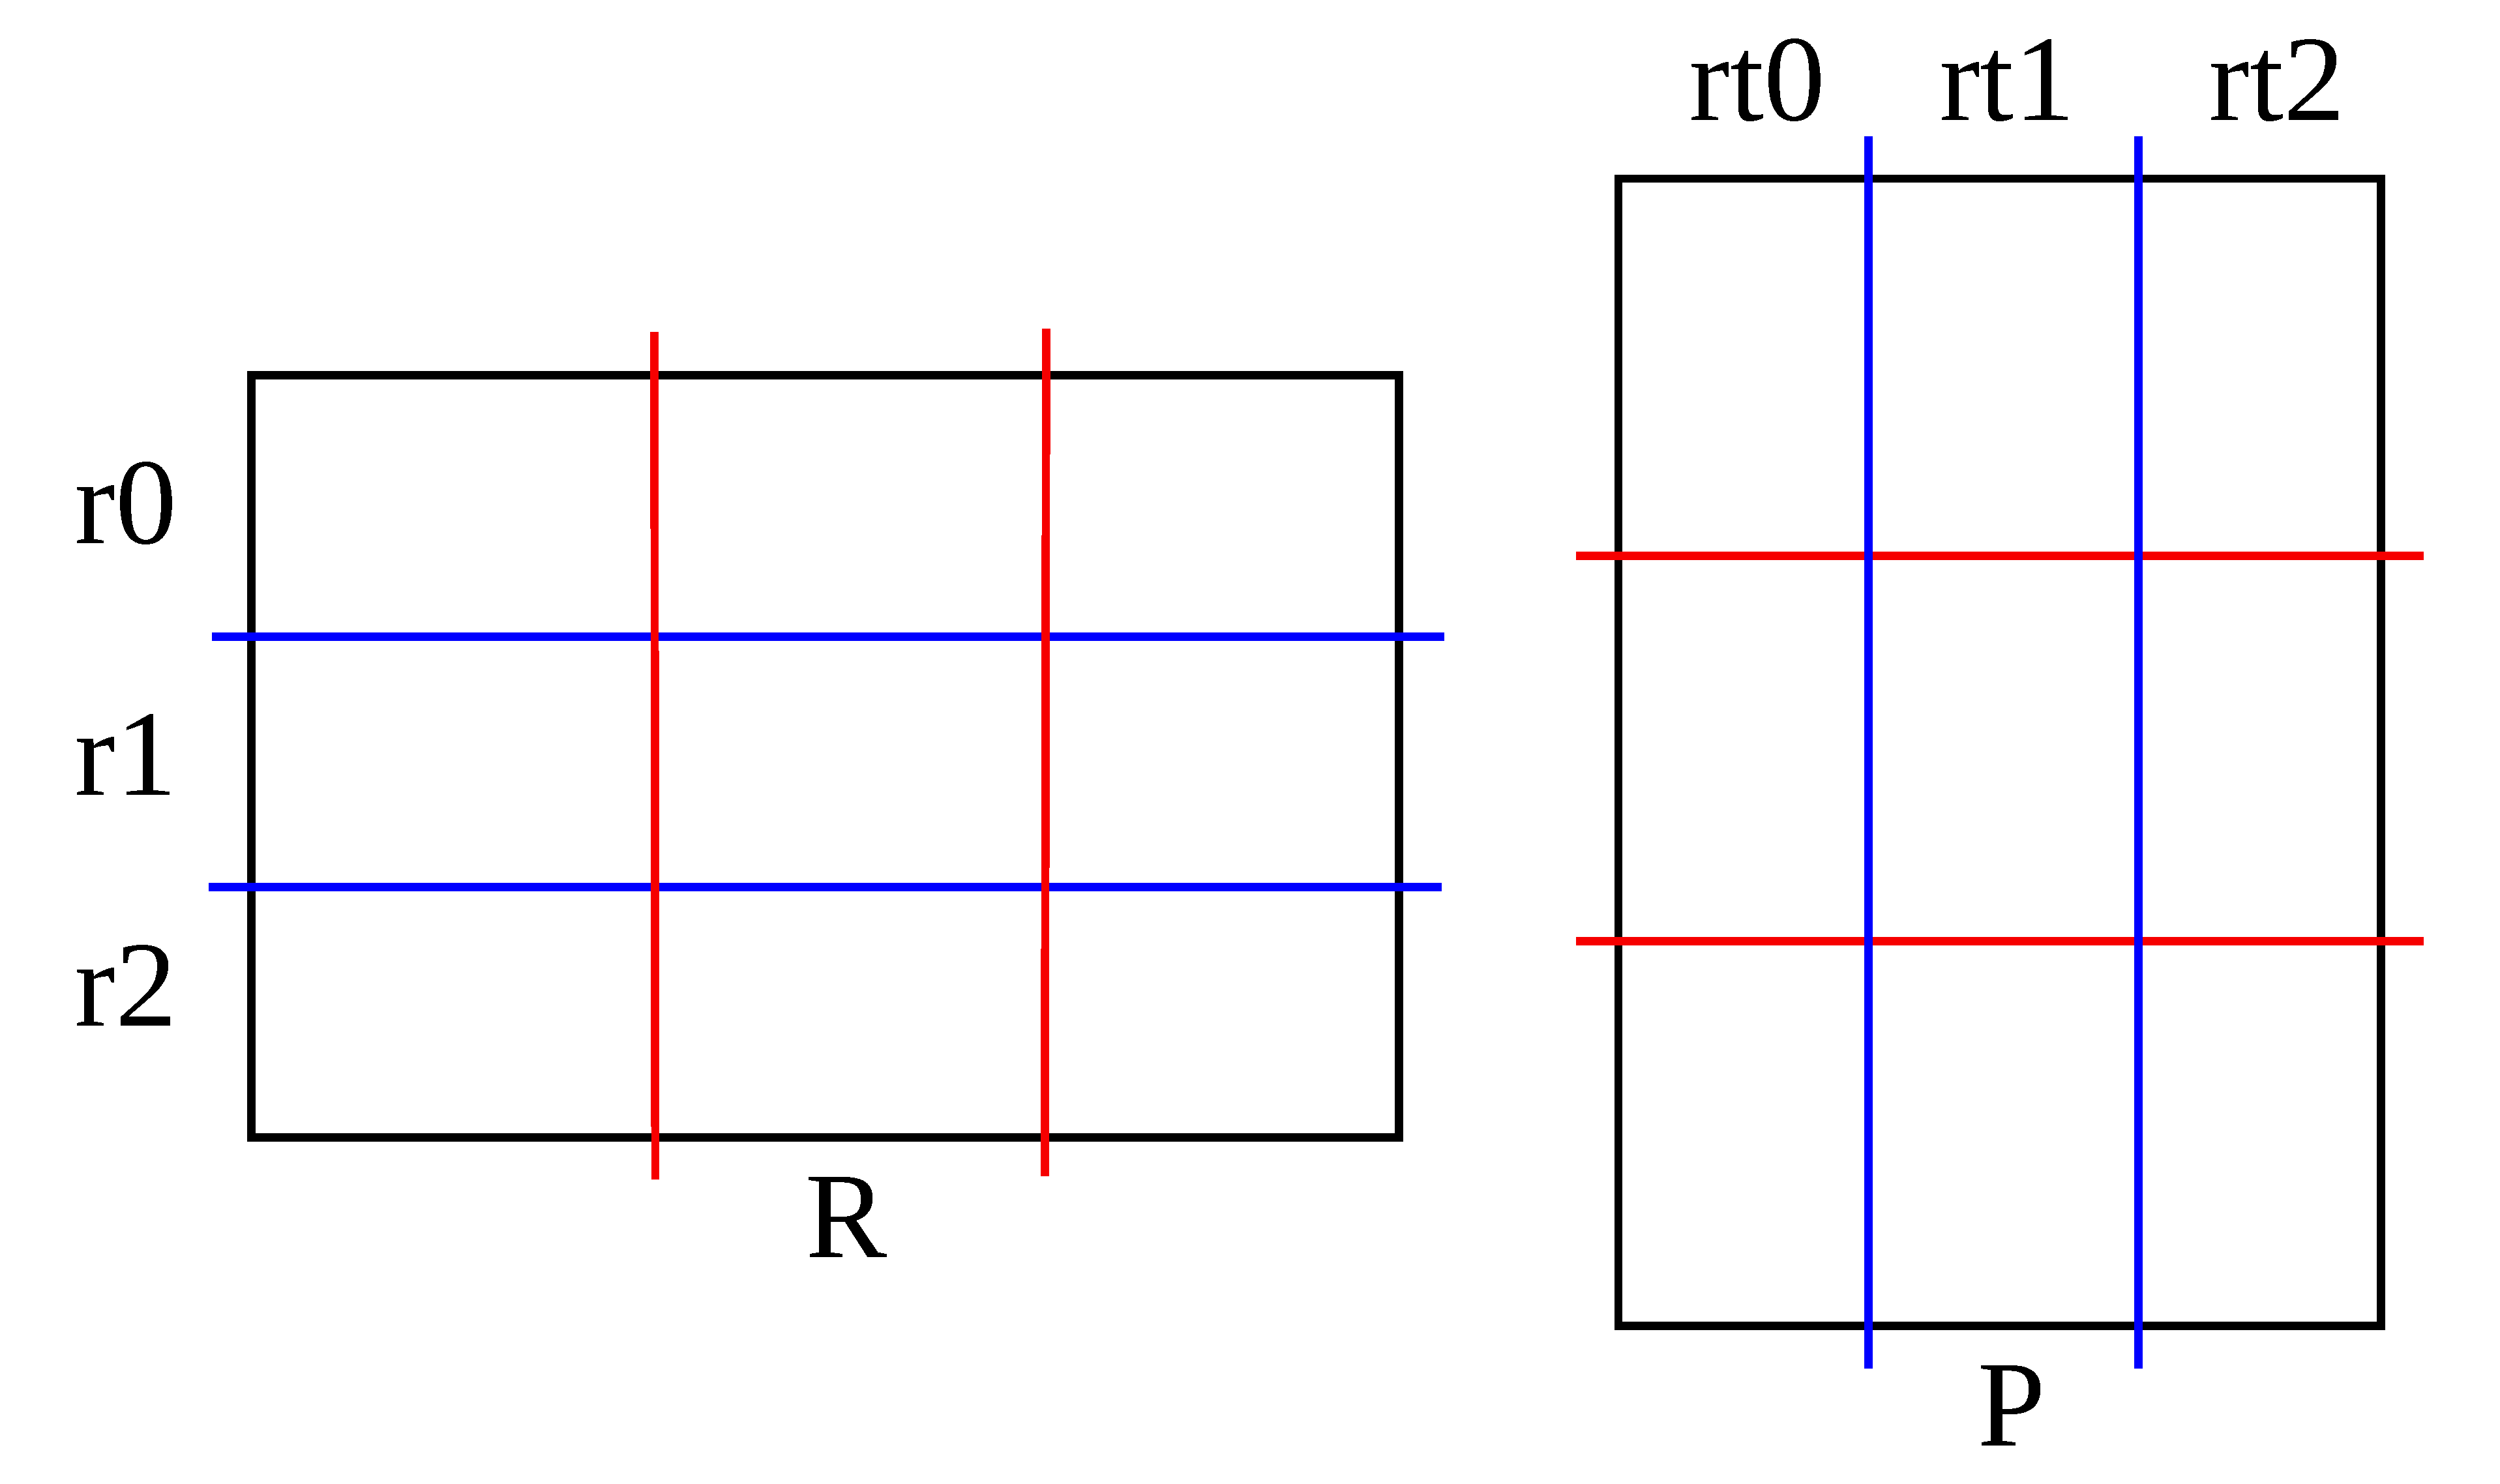
\includegraphics[width=5.5cm,height=3cm]{./figures/part1c.pdf}
 \caption{This figure shows how row blocks of $R$ are transpose of column blocks of $P$.}
 \label{fig:part1c}
\end{figure}
\fi

\begin{algorithm}[H] 
  %\footnotesize
  \caption{Part 1: $B_i = A_i \times P$} \label{alg:part1} 
  \begin{algorithmic}[1]
    \Require $A_i$, $R$
    \Ensure  $B_i$ (result of $A_i \times P$)
    \State $R1 \leftarrow$ transpose of $R_i$ (locally)
    \For{$k=myrank:myrank+nprocs$}
      \State $R2 \leftarrow\ Irecv(transpose\ of\ R block)\ from\ right\ neighbor$
      \State $Isend(R1)\ to\ left\ neighbor$
      \State $B_{ik} \leftarrow \recmm(A_i, R1)$ 
      \State $wait\ for\ Isend\ and\ Irecv\ to\ finish$
      \State $swap(R1,R2)$
    \EndFor
    \State locally sort $B_i$ and add duplicates
  \end{algorithmic}
\end{algorithm}


\subsubsection{Part 2}

Now we explain how to do the second \mm: $R \times B$. The blocks of $R$ on processor $P1$ in, Figure~\ref{fig:part2d}, should be multiplied with the corresponding blocks of $B$ with the same color. In contrary to the previous part, we already don't have the transpose of the right-hand side matrix and performing the transpose in parallel is expensive. Instead, we change the way the multiplication is being done and perform a cheaper communication round at the end.

\begin{figure}[tbh]
    \centering
    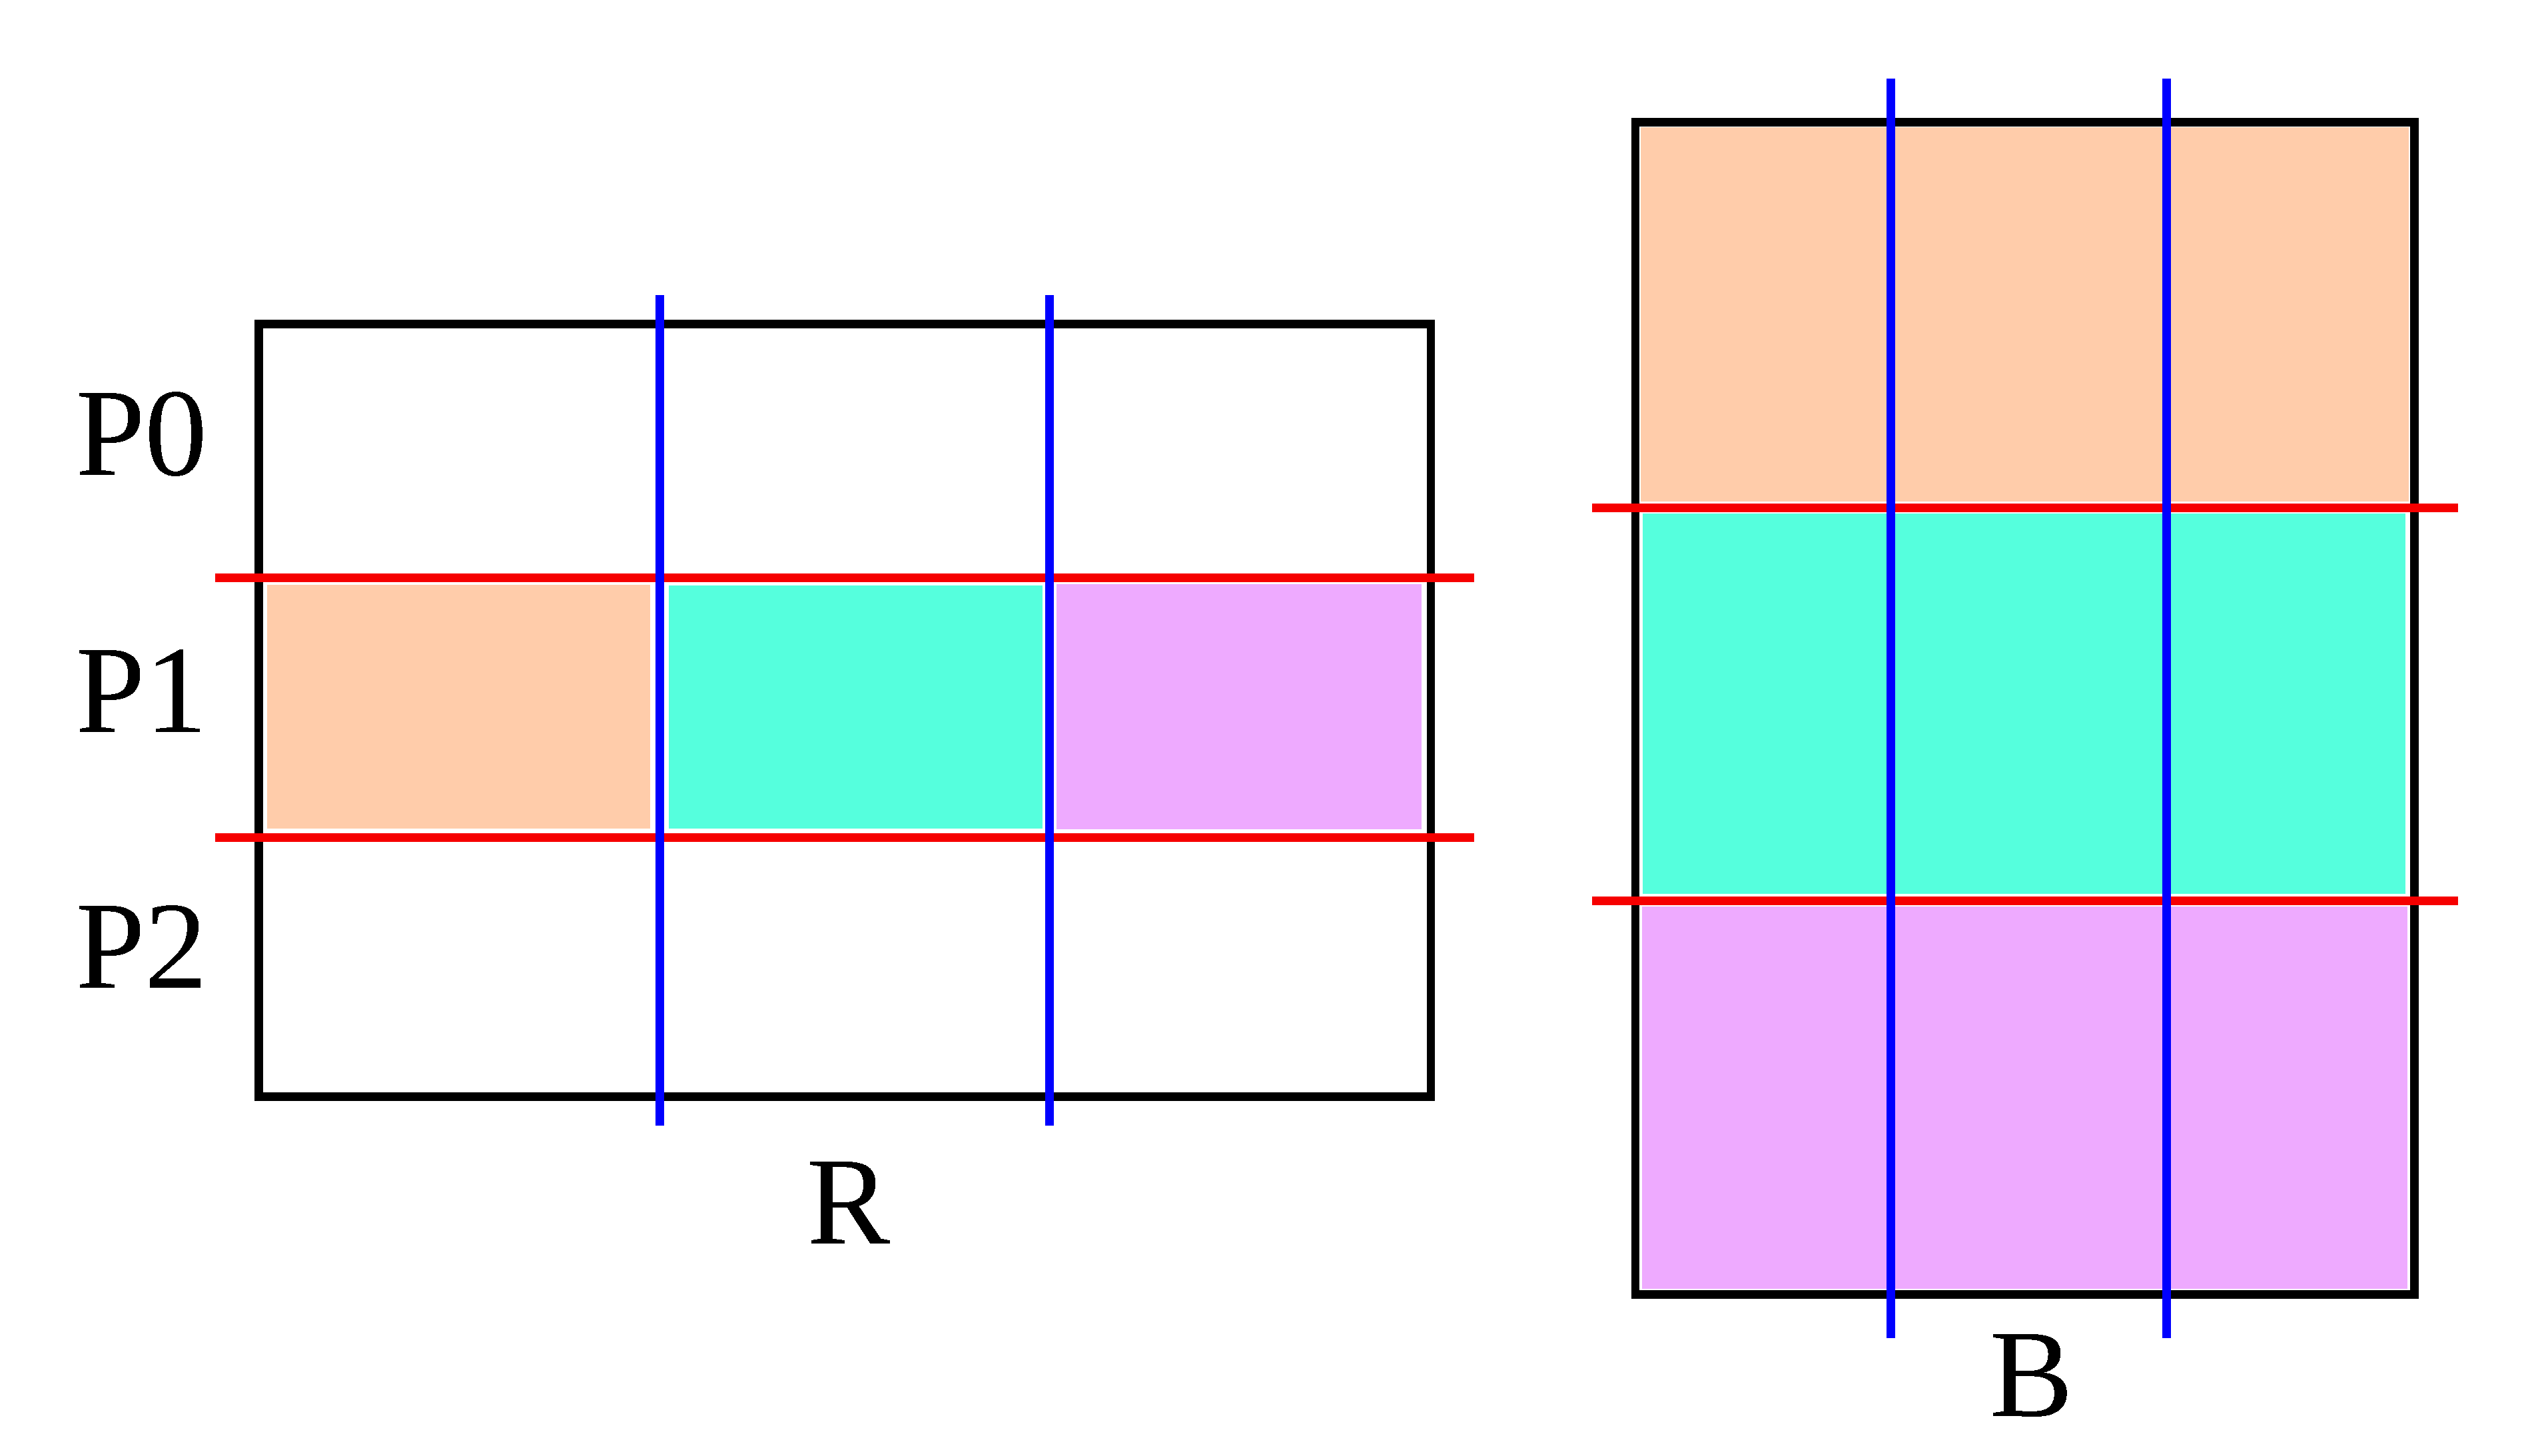
\includegraphics[width=5cm,height=2.8cm]{./figures/part2d.pdf}
    \caption{Part 2: $R \times B$. This figure shows which sub-blocks of R should be multiplied by which sub-blocks of $B$.}
    \label{fig:part2d}
    \Description{}
\end{figure}

\begin{figure}[tbh]
    \centering
    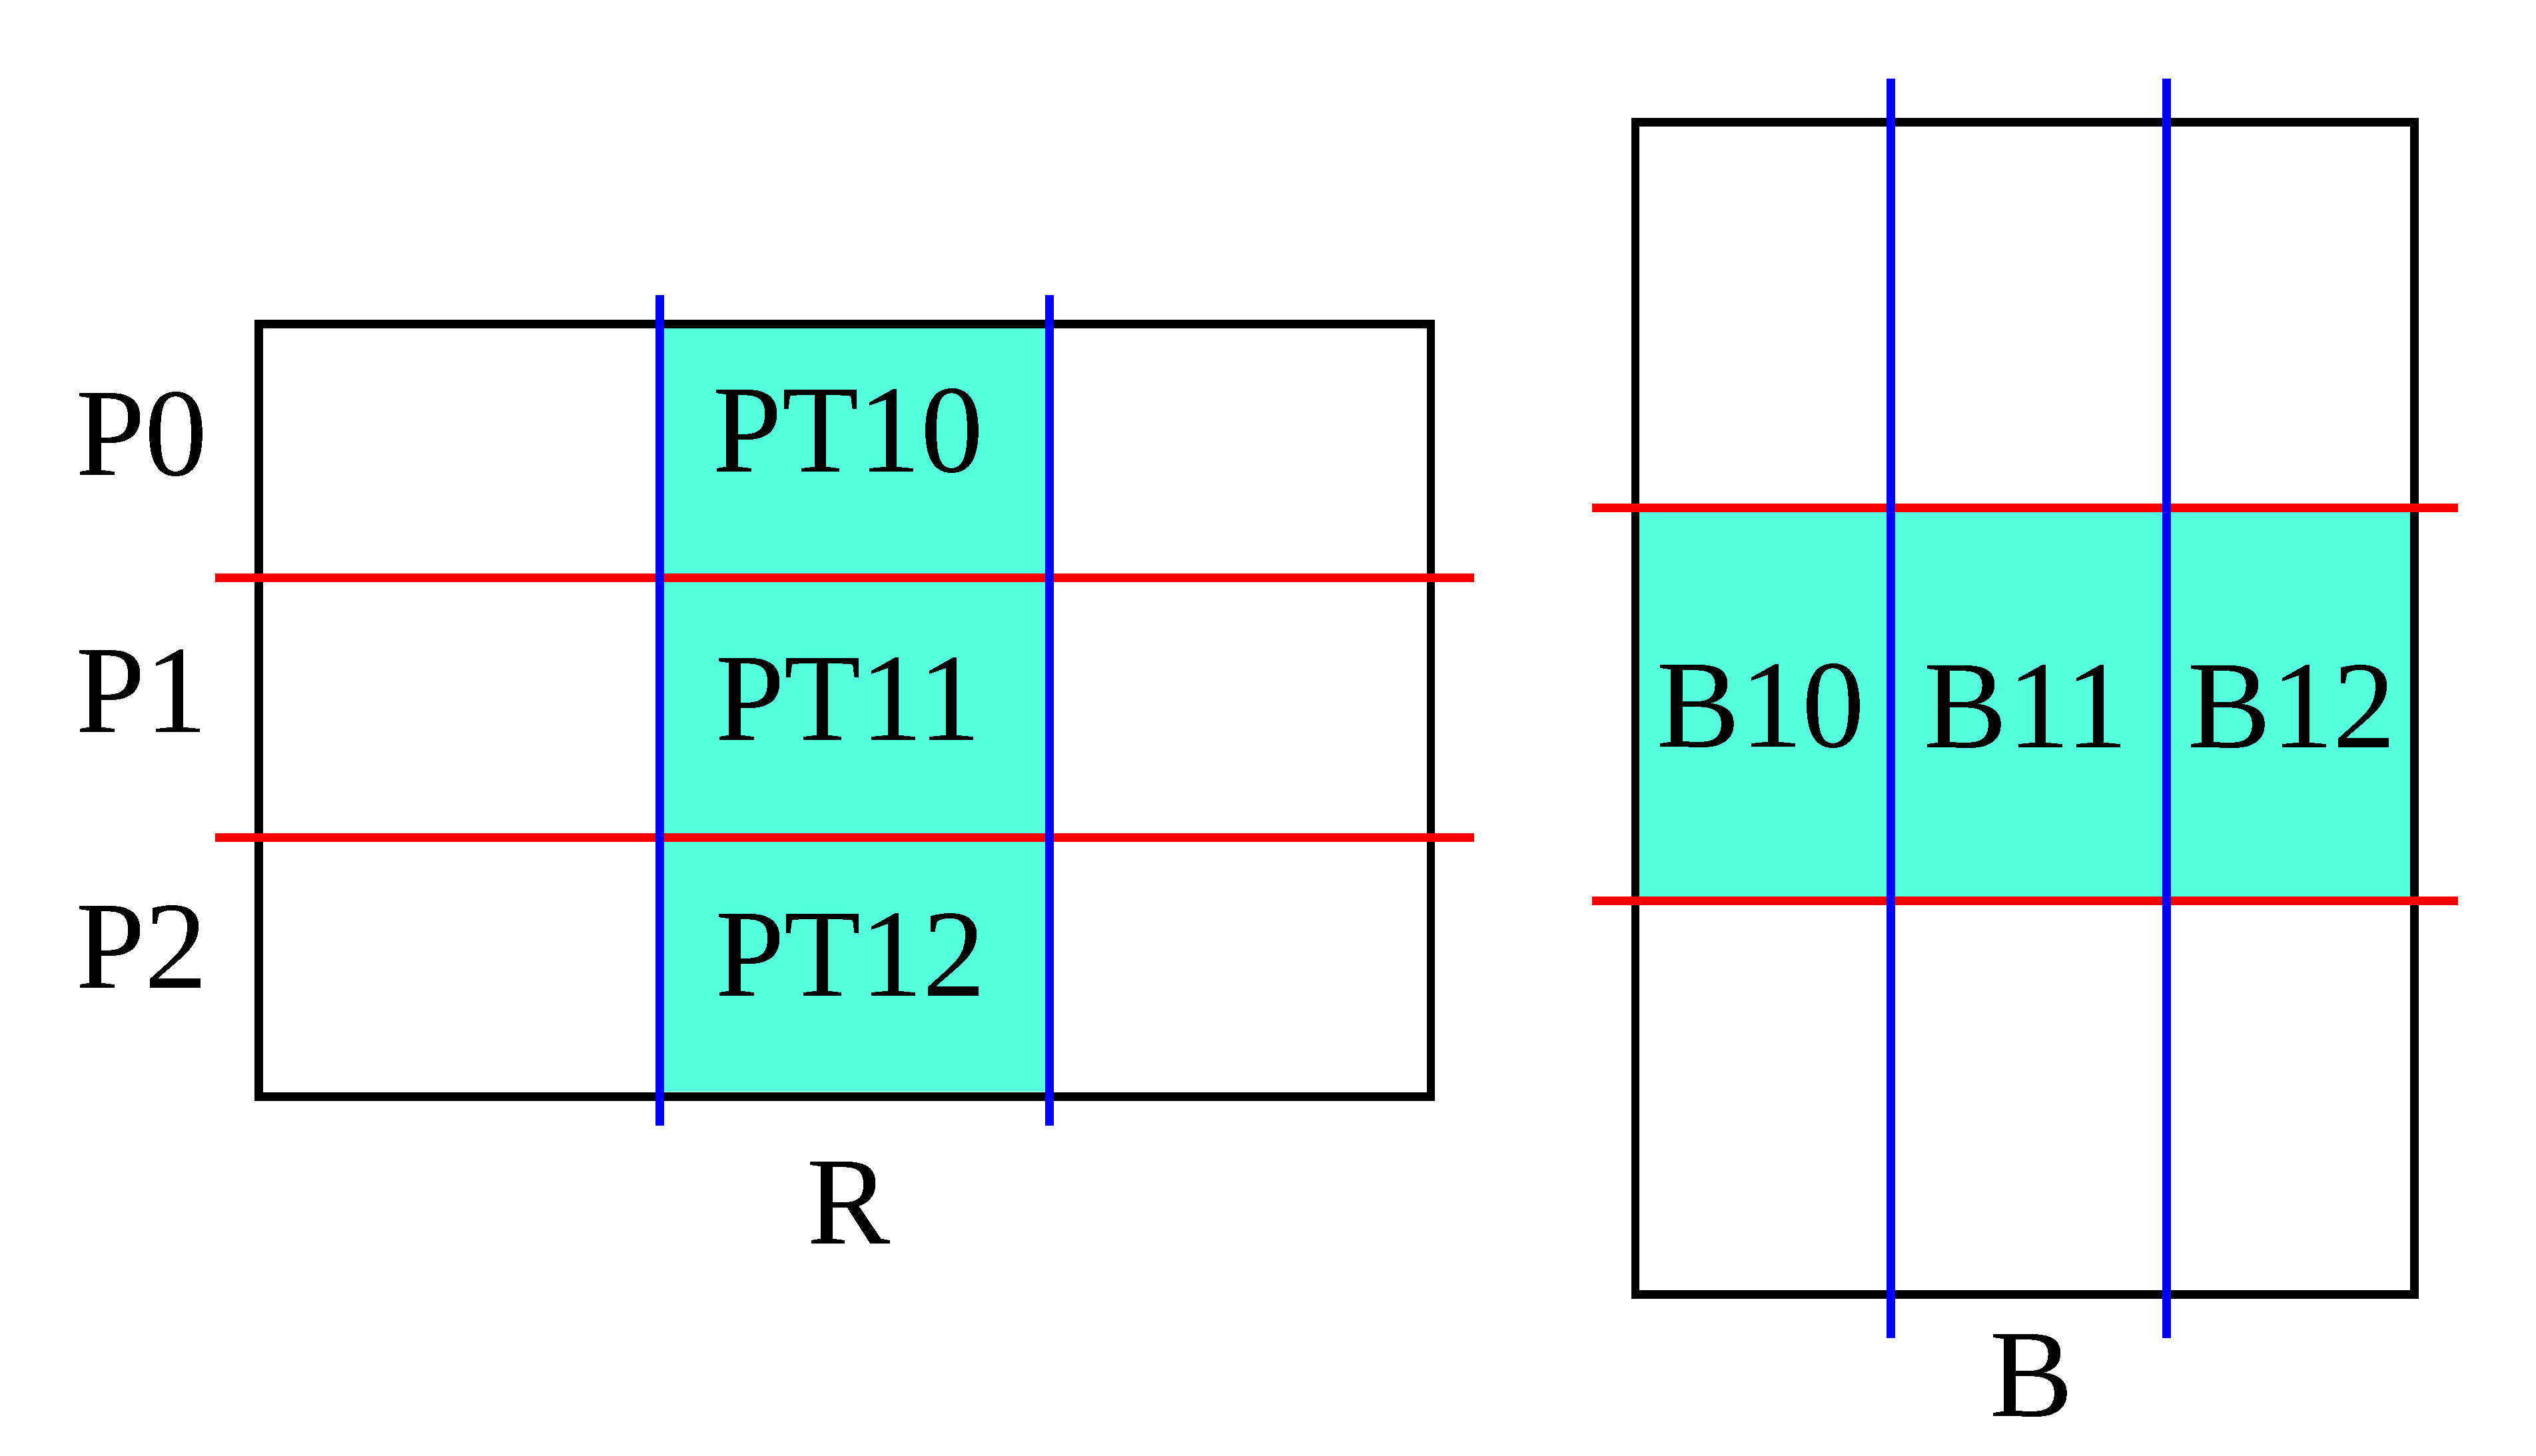
\includegraphics[width=5cm,height=2.8cm]{./figures/part2e.pdf}
    \caption{Local transpose of blocks of $P$ is used instead of $R$. Each green sub-block of the transpose of $P$ is multiplied by all green sub-blocks of $B$.}
    \label{fig:part2e}
    \Description{}
\end{figure}

In this case we have the transpose of the left-hand side matrix, so we use $P$ instead of $R$ to do this multiplication.
We only perform the multiplication of the green blocks on processor $P1$ in Figure~\ref{fig:part2e}, which can be done locally.
%
In the previous case each sub-block of the local left-hand side is multiplied by only one sub-block of the local right-hand side.
But in this method, each sub-block of local $P$ is being multiplied by the entire row block of $B$, e.g. $PT10$ is multiplied by all $B10$, $B11$ and $B12$, and so on.

\iffalse
\begin{figure}[tbh]
 \centering
 %\Description{Description}
 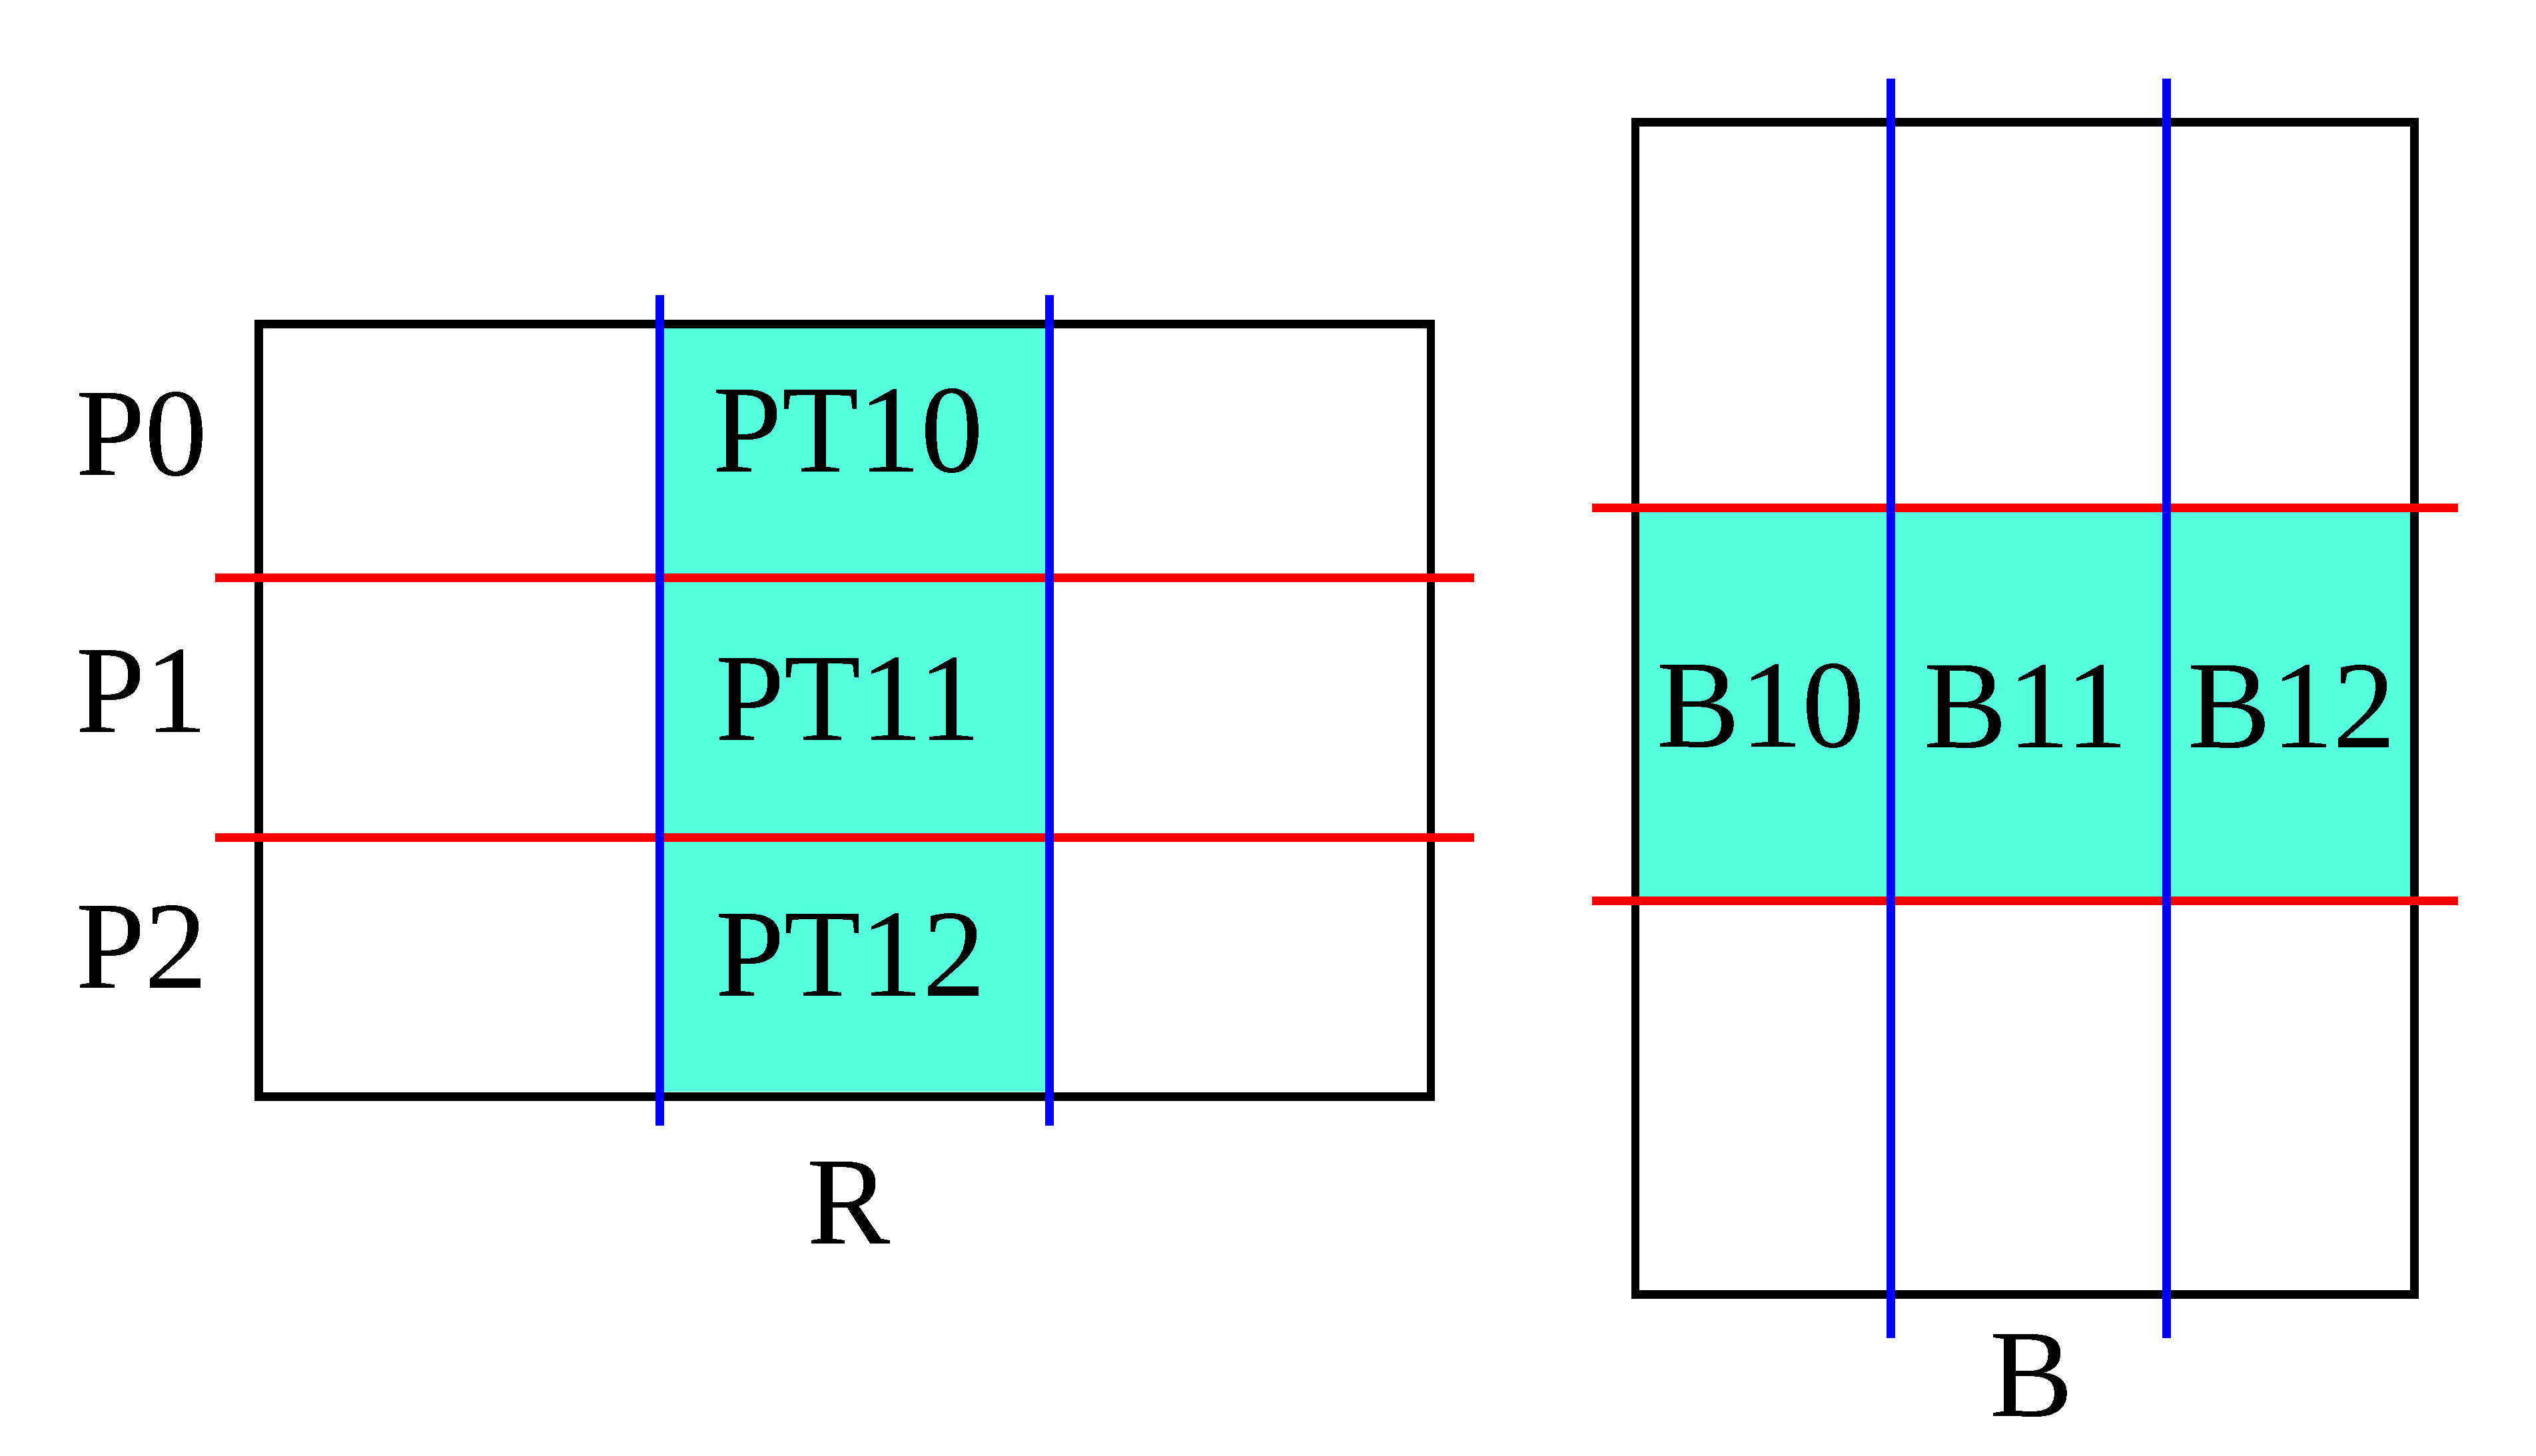
\includegraphics[width=5.5cm,height=3cm]{./figures/part2e.pdf}
 \caption{Local transpose of blocks of $P$ is used instead of $R$. Each green sub-block of the transpose of $P$ is multiplied by all green sub-blocks of $B$.}
 \label{fig:part2e}
\end{figure}
\fi

The difference for final result between this case and the na\"{i}ve Case 2 is that, the final entries are not on the correct processors, so an additional data exchange needs to be performed at the end to restore the entries on the correct processes. We sort the entries locally at the end and add the duplicates together. Finally, we sort them globally (using HykSort \cite{Sundar:2013}) and again add the duplicates together (Algorithm~\ref{alg:part2}).

\begin{algorithm}[H] 
  %\footnotesize
  \caption{Part 2: $Ac = R \times B$} \label{alg:part2} 
  \begin{algorithmic}[1]
    \Require $P_i$, $B_i$
    \Ensure  $Ac_i$
    \State $PT_i \leftarrow$ transpose of $P_i$ (locally)
    \For{$k=0:nprocs$}
      \State $Ac_i \leftarrow \recmm(PT_{ik}, B_i)$
    \EndFor
    \State locally sort $Ac_i$ and add duplicates
    \State globally sort $Ac_i$ and add duplicates
  \end{algorithmic}
\end{algorithm}

Notes:

When doing $A \times B$ in a distributed fashion, it is better to use the local transpose of $B$ for two reasons:

1- After doing each block, sorting and removing duplicates can be done, instead doing that for the whole results.
2- $B$ will be split better. (create a figure for this part)

Explain why CSC is a better option for splitting the matrices. Explain the choice of pivot and the in-place sorting.

Steps for splitting based on CSC:

I) Split Vertically: Reusing row, val from the original block. Modify col-idx by subtracting a fixed number

II) Split Horizontally: 

1- First create col-idx for the bottom and top blocks.

2- Then, perform an in-place sorting by choosing a specifi pivot to change the order for the bottom and top blocks for row and val. Then the bottom and top blocks should have column-major order (because of CSC).
